\documentclass[
  man,
  longtable,
  nolmodern,
  notxfonts,
  notimes,
  colorlinks=true,linkcolor=blue,citecolor=blue,urlcolor=blue]{apa7}

\usepackage{amsmath}
\usepackage{amssymb}




\RequirePackage{longtable}
\RequirePackage{threeparttablex}

\makeatletter
\renewcommand{\paragraph}{\@startsection{paragraph}{4}{\parindent}%
	{0\baselineskip \@plus 0.2ex \@minus 0.2ex}%
	{-.5em}%
	{\normalfont\normalsize\bfseries\typesectitle}}

\renewcommand{\subparagraph}[1]{\@startsection{subparagraph}{5}{0.5em}%
	{0\baselineskip \@plus 0.2ex \@minus 0.2ex}%
	{-\z@\relax}%
	{\normalfont\normalsize\bfseries\itshape\hspace{\parindent}{#1}\textit{\addperi}}{\relax}}
\makeatother




\usepackage{longtable, booktabs, multirow, multicol, colortbl, hhline, caption, array, float, xpatch}
\usepackage{subcaption}
\renewcommand\thesubfigure{\Alph{subfigure}}
\setcounter{topnumber}{2}
\setcounter{bottomnumber}{2}
\setcounter{totalnumber}{4}
\renewcommand{\topfraction}{0.85}
\renewcommand{\bottomfraction}{0.85}
\renewcommand{\textfraction}{0.15}
\renewcommand{\floatpagefraction}{0.7}

\usepackage{tcolorbox}
\tcbuselibrary{listings,theorems, breakable, skins}
\usepackage{fontawesome5}

\definecolor{quarto-callout-color}{HTML}{909090}
\definecolor{quarto-callout-note-color}{HTML}{0758E5}
\definecolor{quarto-callout-important-color}{HTML}{CC1914}
\definecolor{quarto-callout-warning-color}{HTML}{EB9113}
\definecolor{quarto-callout-tip-color}{HTML}{00A047}
\definecolor{quarto-callout-caution-color}{HTML}{FC5300}
\definecolor{quarto-callout-color-frame}{HTML}{ACACAC}
\definecolor{quarto-callout-note-color-frame}{HTML}{4582EC}
\definecolor{quarto-callout-important-color-frame}{HTML}{D9534F}
\definecolor{quarto-callout-warning-color-frame}{HTML}{F0AD4E}
\definecolor{quarto-callout-tip-color-frame}{HTML}{02B875}
\definecolor{quarto-callout-caution-color-frame}{HTML}{FD7E14}

%\newlength\Oldarrayrulewidth
%\newlength\Oldtabcolsep


\usepackage{hyperref}



\usepackage{color}
\usepackage{fancyvrb}
\newcommand{\VerbBar}{|}
\newcommand{\VERB}{\Verb[commandchars=\\\{\}]}
\DefineVerbatimEnvironment{Highlighting}{Verbatim}{commandchars=\\\{\}}
% Add ',fontsize=\small' for more characters per line
\usepackage{framed}
\definecolor{shadecolor}{RGB}{241,243,245}
\newenvironment{Shaded}{\begin{snugshade}}{\end{snugshade}}
\newcommand{\AlertTok}[1]{\textcolor[rgb]{0.68,0.00,0.00}{#1}}
\newcommand{\AnnotationTok}[1]{\textcolor[rgb]{0.37,0.37,0.37}{#1}}
\newcommand{\AttributeTok}[1]{\textcolor[rgb]{0.40,0.45,0.13}{#1}}
\newcommand{\BaseNTok}[1]{\textcolor[rgb]{0.68,0.00,0.00}{#1}}
\newcommand{\BuiltInTok}[1]{\textcolor[rgb]{0.00,0.23,0.31}{#1}}
\newcommand{\CharTok}[1]{\textcolor[rgb]{0.13,0.47,0.30}{#1}}
\newcommand{\CommentTok}[1]{\textcolor[rgb]{0.37,0.37,0.37}{#1}}
\newcommand{\CommentVarTok}[1]{\textcolor[rgb]{0.37,0.37,0.37}{\textit{#1}}}
\newcommand{\ConstantTok}[1]{\textcolor[rgb]{0.56,0.35,0.01}{#1}}
\newcommand{\ControlFlowTok}[1]{\textcolor[rgb]{0.00,0.23,0.31}{\textbf{#1}}}
\newcommand{\DataTypeTok}[1]{\textcolor[rgb]{0.68,0.00,0.00}{#1}}
\newcommand{\DecValTok}[1]{\textcolor[rgb]{0.68,0.00,0.00}{#1}}
\newcommand{\DocumentationTok}[1]{\textcolor[rgb]{0.37,0.37,0.37}{\textit{#1}}}
\newcommand{\ErrorTok}[1]{\textcolor[rgb]{0.68,0.00,0.00}{#1}}
\newcommand{\ExtensionTok}[1]{\textcolor[rgb]{0.00,0.23,0.31}{#1}}
\newcommand{\FloatTok}[1]{\textcolor[rgb]{0.68,0.00,0.00}{#1}}
\newcommand{\FunctionTok}[1]{\textcolor[rgb]{0.28,0.35,0.67}{#1}}
\newcommand{\ImportTok}[1]{\textcolor[rgb]{0.00,0.46,0.62}{#1}}
\newcommand{\InformationTok}[1]{\textcolor[rgb]{0.37,0.37,0.37}{#1}}
\newcommand{\KeywordTok}[1]{\textcolor[rgb]{0.00,0.23,0.31}{\textbf{#1}}}
\newcommand{\NormalTok}[1]{\textcolor[rgb]{0.00,0.23,0.31}{#1}}
\newcommand{\OperatorTok}[1]{\textcolor[rgb]{0.37,0.37,0.37}{#1}}
\newcommand{\OtherTok}[1]{\textcolor[rgb]{0.00,0.23,0.31}{#1}}
\newcommand{\PreprocessorTok}[1]{\textcolor[rgb]{0.68,0.00,0.00}{#1}}
\newcommand{\RegionMarkerTok}[1]{\textcolor[rgb]{0.00,0.23,0.31}{#1}}
\newcommand{\SpecialCharTok}[1]{\textcolor[rgb]{0.37,0.37,0.37}{#1}}
\newcommand{\SpecialStringTok}[1]{\textcolor[rgb]{0.13,0.47,0.30}{#1}}
\newcommand{\StringTok}[1]{\textcolor[rgb]{0.13,0.47,0.30}{#1}}
\newcommand{\VariableTok}[1]{\textcolor[rgb]{0.07,0.07,0.07}{#1}}
\newcommand{\VerbatimStringTok}[1]{\textcolor[rgb]{0.13,0.47,0.30}{#1}}
\newcommand{\WarningTok}[1]{\textcolor[rgb]{0.37,0.37,0.37}{\textit{#1}}}

\providecommand{\tightlist}{%
  \setlength{\itemsep}{0pt}\setlength{\parskip}{0pt}}
\usepackage{longtable,booktabs,array}
\usepackage{calc} % for calculating minipage widths
% Correct order of tables after \paragraph or \subparagraph
\usepackage{etoolbox}
\makeatletter
\patchcmd\longtable{\par}{\if@noskipsec\mbox{}\fi\par}{}{}
\makeatother
% Allow footnotes in longtable head/foot
\IfFileExists{footnotehyper.sty}{\usepackage{footnotehyper}}{\usepackage{footnote}}
\makesavenoteenv{longtable}

\usepackage{graphicx}
\makeatletter
\newsavebox\pandoc@box
\newcommand*\pandocbounded[1]{% scales image to fit in text height/width
  \sbox\pandoc@box{#1}%
  \Gscale@div\@tempa{\textheight}{\dimexpr\ht\pandoc@box+\dp\pandoc@box\relax}%
  \Gscale@div\@tempb{\linewidth}{\wd\pandoc@box}%
  \ifdim\@tempb\p@<\@tempa\p@\let\@tempa\@tempb\fi% select the smaller of both
  \ifdim\@tempa\p@<\p@\scalebox{\@tempa}{\usebox\pandoc@box}%
  \else\usebox{\pandoc@box}%
  \fi%
}
% Set default figure placement to htbp
\def\fps@figure{htbp}
\makeatother


% definitions for citeproc citations
\NewDocumentCommand\citeproctext{}{}
\NewDocumentCommand\citeproc{mm}{%
  \begingroup\def\citeproctext{#2}\cite{#1}\endgroup}
\makeatletter
 % allow citations to break across lines
 \let\@cite@ofmt\@firstofone
 % avoid brackets around text for \cite:
 \def\@biblabel#1{}
 \def\@cite#1#2{{#1\if@tempswa , #2\fi}}
\makeatother
\newlength{\cslhangindent}
\setlength{\cslhangindent}{1.5em}
\newlength{\csllabelwidth}
\setlength{\csllabelwidth}{3em}
\newenvironment{CSLReferences}[2] % #1 hanging-indent, #2 entry-spacing
 {\begin{list}{}{%
  \setlength{\itemindent}{0pt}
  \setlength{\leftmargin}{0pt}
  \setlength{\parsep}{0pt}
  % turn on hanging indent if param 1 is 1
  \ifodd #1
   \setlength{\leftmargin}{\cslhangindent}
   \setlength{\itemindent}{-1\cslhangindent}
  \fi
  % set entry spacing
  \setlength{\itemsep}{#2\baselineskip}}}
 {\end{list}}
\usepackage{calc}
\newcommand{\CSLBlock}[1]{\hfill\break\parbox[t]{\linewidth}{\strut\ignorespaces#1\strut}}
\newcommand{\CSLLeftMargin}[1]{\parbox[t]{\csllabelwidth}{\strut#1\strut}}
\newcommand{\CSLRightInline}[1]{\parbox[t]{\linewidth - \csllabelwidth}{\strut#1\strut}}
\newcommand{\CSLIndent}[1]{\hspace{\cslhangindent}#1}





\usepackage{newtx}

\defaultfontfeatures{Scale=MatchLowercase}
\defaultfontfeatures[\rmfamily]{Ligatures=TeX,Scale=1}





\title{Multivariate analyses of tongue contours from ultrasound tongue
imaging}


\shorttitle{Multivariate analyses of tongue contours from ultrasound
tongue imaging}


\usepackage{etoolbox}








\authorsnames{Stefano Coretta,Georges Sakr}





\affiliation{
{University of Edinburgh}}




\leftheader{Coretta and Sakr}

\date{2025-05-08}


\abstract{This tutorial paper introduces two approaches to modelling
tongue conoutr data obtained with DeepLabCut using Multivariate
Generalised Additive Models (MGAMs) and Multivariate Functional
Principal Component Analysis (MFPCA). For each method, we present a
fully commented analysis of two illustrative data sets: VC
coarticulation in Italian and Polish, and consonant emphaticness in
Lebanese Arabic. All the materials (inlcuding data and code) are
available in the research compendium of the tutorial at
\url{https://github.com/stefanocoretta/mv_uti}. We conclude by
discussing advantages and disadvantages of the two methods (MGAM and
MFPCA) and we recommend researchers to prefer MFPCA over MGAM as an
initial step for modelling tongue contours. }

\keywords{ultrasound tongue imaging, multivariate statistics, functional
principal component analysis, generalised additive
models, phonetics, articulation}

\authornote{\par{\addORCIDlink{Stefano
Coretta}{0000-0001-9627-5532}}\par{\addORCIDlink{Georges
Sakr}{0000-0003-3813-2669}} 

\par{       Author roles were classified using the Contributor Role
Taxonomy (CRediT; https://credit.niso.org/) as follows:  Stefano
Coretta:   conceptualisation, data
curation, methodology, software, supervision, validation, visualisation, writing, editing; Georges
Sakr:   data curation, methodology, writing, editing}
\par{Correspondence concerning this article should be addressed
to Stefano
Coretta, Email: \href{mailto:s.coretta@ed.ac.uk}{s.coretta@ed.ac.uk}}
}

\makeatletter
\let\endoldlt\endlongtable
\def\endlongtable{
\hline
\endoldlt
}
\makeatother
\RequirePackage{longtable}
\DeclareDelayedFloatFlavor{longtable}{table}

\urlstyle{same}



\makeatletter
\@ifpackageloaded{tcolorbox}{}{\usepackage[skins,breakable]{tcolorbox}}
\@ifpackageloaded{fontawesome5}{}{\usepackage{fontawesome5}}
\definecolor{quarto-callout-color}{HTML}{909090}
\definecolor{quarto-callout-note-color}{HTML}{0758E5}
\definecolor{quarto-callout-important-color}{HTML}{CC1914}
\definecolor{quarto-callout-warning-color}{HTML}{EB9113}
\definecolor{quarto-callout-tip-color}{HTML}{00A047}
\definecolor{quarto-callout-caution-color}{HTML}{FC5300}
\definecolor{quarto-callout-color-frame}{HTML}{acacac}
\definecolor{quarto-callout-note-color-frame}{HTML}{4582ec}
\definecolor{quarto-callout-important-color-frame}{HTML}{d9534f}
\definecolor{quarto-callout-warning-color-frame}{HTML}{f0ad4e}
\definecolor{quarto-callout-tip-color-frame}{HTML}{02b875}
\definecolor{quarto-callout-caution-color-frame}{HTML}{fd7e14}
\makeatother
\makeatletter
\@ifpackageloaded{caption}{}{\usepackage{caption}}
\AtBeginDocument{%
\ifdefined\contentsname
  \renewcommand*\contentsname{Table of contents}
\else
  \newcommand\contentsname{Table of contents}
\fi
\ifdefined\listfigurename
  \renewcommand*\listfigurename{List of Figures}
\else
  \newcommand\listfigurename{List of Figures}
\fi
\ifdefined\listtablename
  \renewcommand*\listtablename{List of Tables}
\else
  \newcommand\listtablename{List of Tables}
\fi
\ifdefined\figurename
  \renewcommand*\figurename{Figure}
\else
  \newcommand\figurename{Figure}
\fi
\ifdefined\tablename
  \renewcommand*\tablename{Table}
\else
  \newcommand\tablename{Table}
\fi
}
\@ifpackageloaded{float}{}{\usepackage{float}}
\floatstyle{ruled}
\@ifundefined{c@chapter}{\newfloat{codelisting}{h}{lop}}{\newfloat{codelisting}{h}{lop}[chapter]}
\floatname{codelisting}{Listing}
\newcommand*\listoflistings{\listof{codelisting}{List of Listings}}
\makeatother
\makeatletter
\makeatother
\makeatletter
\@ifpackageloaded{caption}{}{\usepackage{caption}}
\@ifpackageloaded{subcaption}{}{\usepackage{subcaption}}
\makeatother

% From https://tex.stackexchange.com/a/645996/211326
%%% apa7 doesn't want to add appendix section titles in the toc
%%% let's make it do it
\makeatletter
\xpatchcmd{\appendix}
  {\par}
  {\addcontentsline{toc}{section}{\@currentlabelname}\par}
  {}{}
\makeatother

%% Disable longtable counter
%% https://tex.stackexchange.com/a/248395/211326

\usepackage{etoolbox}

\makeatletter
\patchcmd{\LT@caption}
  {\bgroup}
  {\bgroup\global\LTpatch@captiontrue}
  {}{}
\patchcmd{\longtable}
  {\par}
  {\par\global\LTpatch@captionfalse}
  {}{}
\apptocmd{\endlongtable}
  {\ifLTpatch@caption\else\addtocounter{table}{-1}\fi}
  {}{}
\newif\ifLTpatch@caption
\makeatother

\begin{document}

\maketitle


\setcounter{secnumdepth}{-\maxdimen} % remove section numbering

\setlength\LTleft{0pt}


\section{Introduction}\label{introduction}

Ultrasound Tongue Imaging (UTI) is a non-invasive technique that allows
researchers to image the shape of the tongue during speech at medium
temporal resolution (30-100 frames per second,
\citeproc{ref-epstein2005}{Epstein \& Stone, 2005};
\citeproc{ref-stone2005}{Stone, 2005}). Typically, the midsagittal
contour of the tongue is imaged, although 3D systems exist
(\citeproc{ref-lulich2018}{Lulich et al., 2018}). Recent developments in
machine learning assisted image processing has enabled faster tracking
of estimated points on the tongue contour
(\citeproc{ref-wrench2022}{Wrench \& Balch-Tomes, 2022}).

Wrench and Balch-Tomes (\citeproc{ref-wrench2022}{2022}) have trained a
DeepLabCut (DLC, \citeproc{ref-mathis2018}{Mathis et al., 2018}) model
to estimate and track specific flesh points on the tongue contour and
anatomical landmarks as captured by UTI. The model estimates 11
``knots'' from the vallecula to the tongue tip, plus three
muscular-skeletal knots (the hyoid bone, the mandible base and the
mental spine where the short tendon attaches). See
Figure~\ref{fig-knots} for a schematic illustration of the position of
the tracked knots. An advantage of DLC-tracked data over the traditional
fan-line coordinate system is that (in theory) specific (moving) flesh
points are tracked rather than simply the intersection of the tongue
contour with fixed radii from the fan-line system. This makes
DLC-tracked data resemble data obtained with electromagnetic
articulography (EMA). The downside is that the tongue contour is
represented by 11 freely moving points, which can move in any direction
in the midsagittal two-dimensional space captured by UTI.

\begin{figure}

\caption{\label{fig-knots}Schematic representation of the knots tracked
by DeepLabCut. CC-BY Wrench and Balch-Tomes
(\citeproc{ref-wrench2024}{Wrench, 2024}).}

\centering{

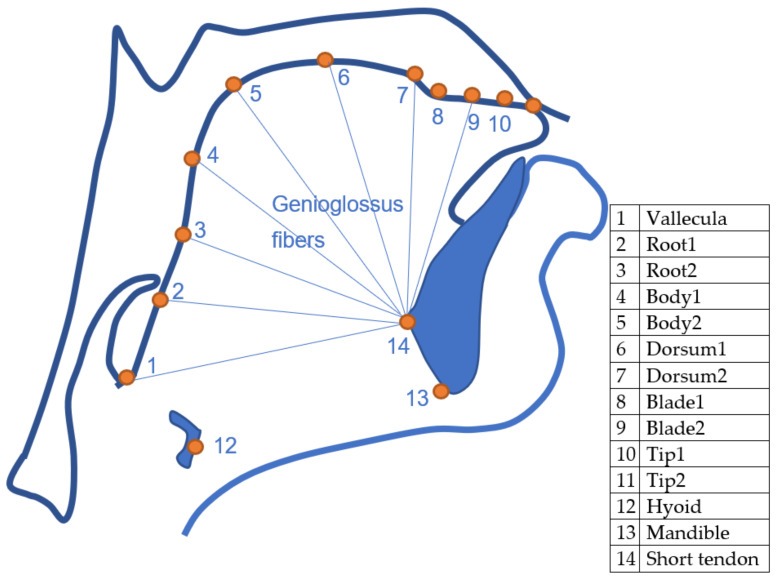
\includegraphics[width=5.20833in,height=\textheight,keepaspectratio]{img/sensors-22-01133-g002.jpg}

}

\end{figure}%

Classical ways to analyse tongue contour data obtained from a fan-line
system, like SS-ANOVA (\citeproc{ref-chen2011}{Chen \& Lin, 2011};
\citeproc{ref-davidson2006}{Davidson, 2006}) and Generalised Additive
Models using polar coordinates (\citeproc{ref-coretta2019g}{Coretta,
n.d.}, \citeproc{ref-coretta2018c}{2018b}), are not appropriate with
DLC-tracked data, due to the tongue contour ``curling'' onto itself
along the root. This is illustrated in Figure~\ref{fig-curl}: the plot
shows the DLC-tracked points (in black) of the data from a Polish
speaker and the traced tongue contours based on the points (see
Section~\ref{sec-gam-vc-coart} for details on the data). The contours
clearly curl onto themselves along the root (on the left of the
contour). The red smooths represent a LOESS smooth, calculated for Y
along X. This approach clearly miscalculates the smooth for the back
half of the tongue, simply because there are two Y values for the same X
value, and the procedure, in that case, returns something like an
average of the two values. Generalised Additive Models (introduced in
the following section) work on the same principle and hence would
produce the same type of error. Using polar coordinates would not solve
the problem: while a fan-line system lends itself easily to using polar
coordinates (since the origin of the probe can be used to approximate
the origin of the coordinate system), this cannot be done with DLC data
because there is no single origin in the actual tongue anatomy from
which vectors of displacement radiate, that would work for all tracked
points.

\phantomsection\label{cell-fig-curl}
\begin{figure}[H]

\caption{\label{fig-curl}Illustrating tongue contours curling up along
the root. The estimated smooths in red fail to capture the curl.}

\centering{

\pandocbounded{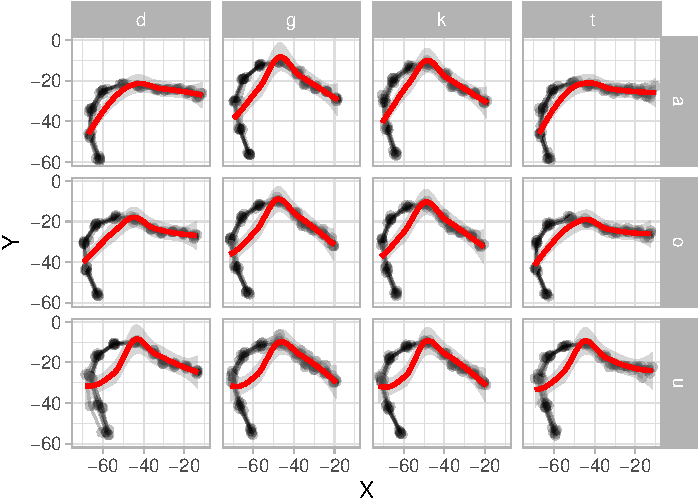
\includegraphics[keepaspectratio]{index_files/figure-pdf/fig-curl-1.pdf}}

}

\end{figure}%

In this tutorial, we introduce two alternative methods to analyse
DLC-tracked tongue contour data: Multivariate Generalised Additive
Models (Section~\ref{sec-gam}) and Multivariate Functional Principal
Component Analysis (Section~\ref{sec-fpca}). We will present the pros
and cons of each method in Section~\ref{sec-procons}, but to summarise
we are inclined to recommend Multivariate Functional Principal Component
Analysis over Multivariate Generalised Additive Models due to the
substantial computational overhead and reduced practical utility of the
latter over the former.

\section{Multivariate Generalised Additive Models}\label{sec-gam}

Generalised Additive Models (GAMs) are an extension of generalised
models that allow flexible modelling of non-linear effects
(\citeproc{ref-hastie1986}{Hastie \& Tibshirani, 1986};
\citeproc{ref-wood2006}{Wood, 2006}). GAMs are built upon smoothing
splines functions, the components of which are multiplied by estimated
coefficients to reconstruct an arbitrary time-changing curve. For a
thorough introduction to GAMs we refer the reader to Sóskuthy
(\citeproc{ref-soskuthy2017a}{2021b}); Sóskuthy
(\citeproc{ref-soskuthy2021}{2021a}); Pedersen et al.
(\citeproc{ref-pedersen2019}{2019}); Wieling
(\citeproc{ref-wieling2018}{2018}). Multivariate Generalised Additive
Models (MGAMs) are GAMs with more than one outcome variable.

As mentioned in the Introduction, the data tracked by DeepLabCut
consists of the position on the horizontal (\emph{x}) and vertical
(\emph{y}) axes of fourteen knots. In this tutorial, we will focus on
modelling the tongue contour based on the 11 knots from the vallecula to
the tongue tip. Figure~\ref{fig-tongue} illustrates the reconstructed
tongue contour on the basis of the 11 knots: the shown tongue is from
the offset of a vowel {[}o{]} followed by {[}t{]}, uttered by a Polish
speaker (see Section~\ref{sec-gam-vc-coart}).

\phantomsection\label{cell-fig-tongue}
\begin{figure}[H]

\caption{\label{fig-tongue}The eleven knots on the tongue contour taken
from the offset of {[}o{]} followed by {[}t{]} (Polish speaker PL04,
tongue tip to the right).}

\centering{

\pandocbounded{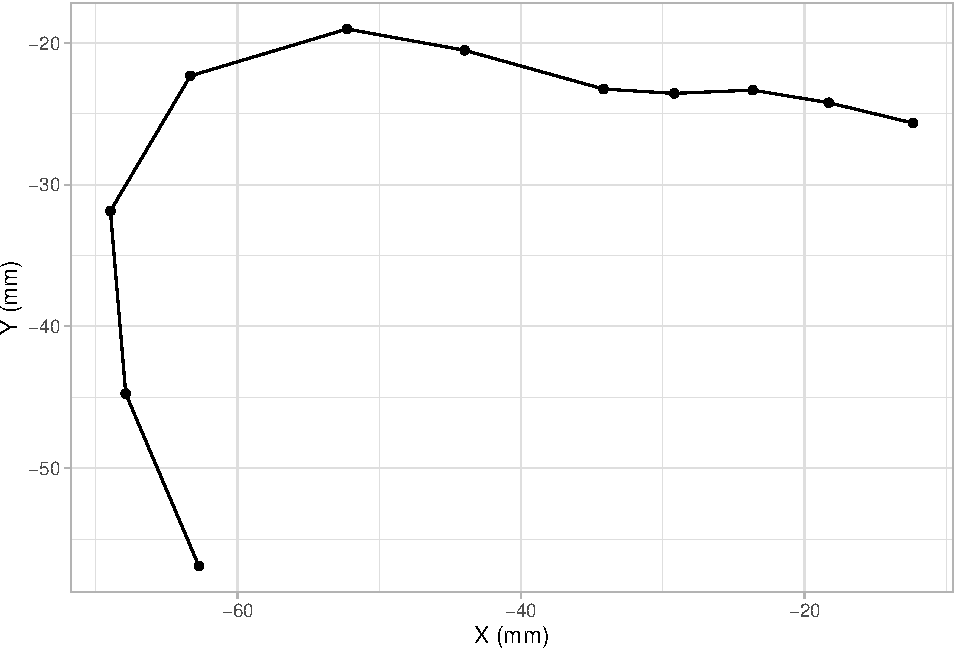
\includegraphics[keepaspectratio]{index_files/figure-pdf/fig-tongue-1.pdf}}

}

\end{figure}%

The same data is shown in Figure~\ref{fig-tongue-xy} in a different
format. Instead of a Cartesian coordinate system of X and Y values, the
plot has knot number on the \emph{x}-axis and X/Y coordinates on the
\emph{y}-axis. The X/Y coordinates thus form ``trajectories'' along the
knots. These X/Y trajectories are the ones that can be modelled using
MGAMs and Multiple Functional Principal Component Analysis (MFPCA): in
both cases, the X/Y trajectories are modelled as two variables changing
along knot number. In this section, we will illustrate GAMs applied to
the X/Y trajectories along the knots and how we can reconstruct the
tongue contour from the modelled trajectories. We will use data from two
case studies of coarticulation: vowel consonant (VC) coarticulation
based on C place in Italian and Polish, and consonantal articulation of
plain vs emphatic consonants in Lebanese Arabic.

\phantomsection\label{cell-fig-tongue-xy}
\begin{figure}[H]

\caption{\label{fig-tongue-xy}The horizontal and vertical positions of
the elevel knots (same data as Figure~\ref{fig-tongue}).}

\centering{

\pandocbounded{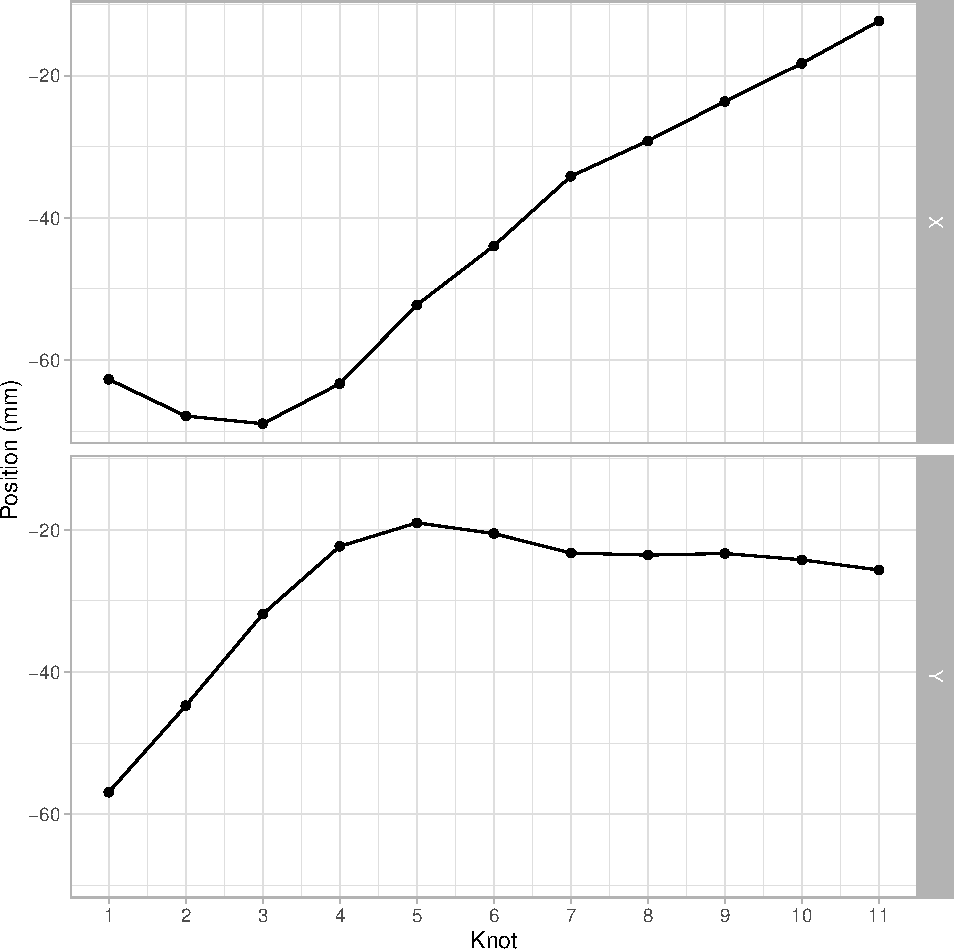
\includegraphics[keepaspectratio]{index_files/figure-pdf/fig-tongue-xy-1.pdf}}

}

\end{figure}%

\subsection{VC coarticulation}\label{sec-gam-vc-coart}

The data of the first case study, Coretta
(\citeproc{ref-coretta2018f}{2018a}), comes from Coretta
(\citeproc{ref-coretta2020b}{2020b}) and has been discussed in Coretta
(\citeproc{ref-coretta2020}{2020a}) (the analysis concerned the position
of the tongue root during the duration of vowels followed by voiceless
or voiced stops; in this paper we focus on tongue contours at the vowel
offset). The materials are /pVCV/ words embedded in a frame sentence
(\emph{Dico X lentamente} `I say X slowly' in Italian and \emph{Mówię X
teraz} `I say X now' in Polish). In the /pVCV/ words, C was /t, d, k, ɡ/
and V was /a, o, u/ (in each word, the two vowels were identical, so for
example \emph{pata, poto, putu}). The data analysed here is from 9
speakers of Italian and 6 speakers of Polish (other speakers were not
included due to the difficulty in processing their data with
DeepLabCut).

Video recordings of tongue ultrasound were obtained in Articulate
Assistant Advanced™ (AAA, \citeproc{ref-ltd2011}{Articulate Instruments
Ldt., 2011}). Spline data was extracted using a custom DeepLabCut (DLC)
model developed by Wrench and Balch-Tomes
(\citeproc{ref-wrench2022}{2022}). When exporting from AAA™, the data
was rotated based on the bite plane, obtained with the imaging of a bite
plate (\citeproc{ref-scobbie2011}{Scobbie et al., 2011}), so that the
bite plane is horizontal: this allows for a common coordinate system
where vertical and horizontal movement are comparable across speakers.
Once the DLC data was imported in R, we manually removed tracking errors
and we calculated \emph{z}-scores within each speaker (the difference
between the value and the mean, divided by the standard deviation).
These steps are documented in the paper's notebook
\href{notebooks/01_prepare_data.qmd}{Prepare data}.

The following code chunk reads the filtered data. A sample of the data
is shown in Table~\ref{tbl-dlc-voff}. Figure~\ref{fig-voff} shows the
tongue contours for each individual speaker. It is possible to notice
clusters of different contours, related to each of the vowels /a, o, u/.
Figure~\ref{fig-pl04} zooms in on PL04 (Polish): the contours of each
vowel are coloured separately, and two panels separate tongue contours
taken at the offset of vowels followed by coronal (/t, d/) and velar
stops (/k, ɡ/). Crucially, the variation in tongue shape at vowel offset
(or closure onset) across vowels contexts is higher in the coronal than
in the velar contexts. This is not surprising, giving the greater
involvement of the tongue body and dorsum (the relevant articulators of
vowel production) in velar than in coronal stops.

\begin{Shaded}
\begin{Highlighting}[]
\NormalTok{dlc\_voff\_f }\OtherTok{\textless{}{-}} \FunctionTok{readRDS}\NormalTok{(}\StringTok{"data/coretta2018/dlc\_voff\_f.rds"}\NormalTok{)}
\end{Highlighting}
\end{Shaded}

\begin{table}

{\caption{{A sample of the VC coarticulation data from Coretta
(\citeproc{ref-coretta2018f}{2018a}).}{\label{tbl-dlc-voff}}}
\vspace{-20pt}}

\begin{longtable}[]{@{}llrrrl@{}}
\toprule\noalign{}
speaker & word & X & Y & knot & knot\_label \\
\midrule\noalign{}
\endhead
\bottomrule\noalign{}
\endlastfoot
it01 & pugu & -55.2105 & -44.1224 & 0 & Vallecula \\
it01 & pugu & -60.6994 & -31.3486 & 1 & Root\_1 \\
it01 & pugu & -65.1434 & -17.7311 & 2 & Root\_2 \\
it01 & pugu & -63.6757 & -4.2022 & 3 & Body\_1 \\
it01 & pugu & -57.2505 & 7.8483 & 4 & Body\_2 \\
it01 & pugu & -44.9086 & 13.3162 & 5 & Dorsum\_1 \\
\end{longtable}

\end{table}

\phantomsection\label{cell-fig-voff}
\begin{figure}[H]

\caption{\label{fig-voff}Tongue contours of 9 Italian speakers and6
Polish speakers, taken from the offset of the first vowel in /pCVCV/
target words.}

\centering{

\pandocbounded{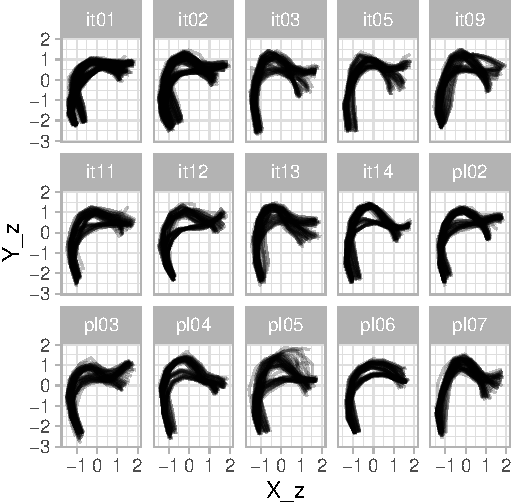
\includegraphics[keepaspectratio]{index_files/figure-pdf/fig-voff-1.pdf}}

}

\end{figure}%

\phantomsection\label{cell-fig-pl04}
\begin{figure}[H]

\caption{\label{fig-pl04}Tongue contours of PL04 (Polish) taken from the
offset of vowels followed by coronal or velar stops. Tip is on the
right.}

\centering{

\pandocbounded{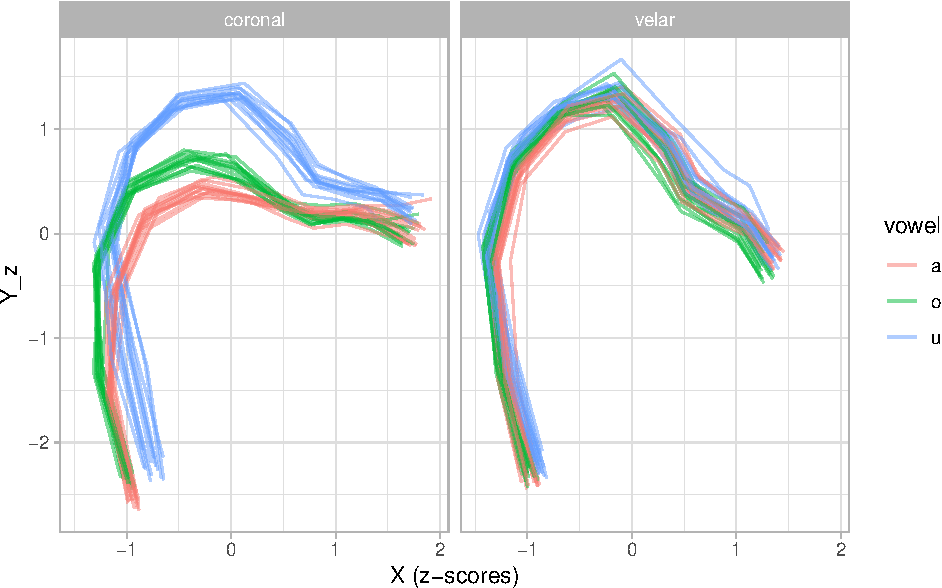
\includegraphics[keepaspectratio]{index_files/figure-pdf/fig-pl04-1.pdf}}

}

\end{figure}%

We can now run a multivariate GAM to model the tongue contours. A
multivariate GAM can be fitted by providing model formulae for each
outcome variable (in our case, \texttt{X\_z} and \texttt{Y\_z}) in a
list. For example
\texttt{list(y\ \textasciitilde{}\ s(x),\ w\ \textasciitilde{}\ s(x))}
would instruct \texttt{mgcv::gam()} to fit a bivariate GAM with the two
outcome variables \texttt{y} and \texttt{w}. The required family is
\texttt{mvn} for ``multivariate normal'': \texttt{mvn(d\ =\ 2)}
indicates a bivariate family (a multivariate family with two dimensions,
i.e.~two outcome variables). In the model below, we are fitting a
multivariate GAM to the \emph{z}-scored X and Y coordinates. For both
outcome variables, we include a smooth over knot
(\texttt{s(knot,\ ...)}) with a \texttt{by} variable
\texttt{vow\_place\_lang}: this variable is built from an interaction of
vowel, place and language.\footnote{Note that interactions between
  categorical variables in the classical sense are not possible in GAMs.
  Instead, one can approximate interactions by creating an ``interaction
  variable'', which is simply a variable where the values of the
  interacting variables are pasted together.} We set \texttt{k} to 5:
this will usually be sufficient for X/Y coordinates of tongue contours,
since they are by nature not very ``wiggly'' (which would require a
higher \texttt{k}). We also include a factor smooth over knot for
speaker (the equivalent of a non-linear random effect) with
\texttt{s(knot,\ speaker,\ ...)}: since language is a between-speaker
variable, we use the interaction of vowel and place,
\texttt{vow\_place}, as the \texttt{by} variable.

\begin{Shaded}
\begin{Highlighting}[]
\FunctionTok{library}\NormalTok{(mgcv)}

\NormalTok{voff\_gam }\OtherTok{\textless{}{-}} \FunctionTok{gam}\NormalTok{(}
  \FunctionTok{list}\NormalTok{(}
\NormalTok{    X\_z }\SpecialCharTok{\textasciitilde{}}\NormalTok{ vow\_place\_lang }\SpecialCharTok{+}
      \FunctionTok{s}\NormalTok{(knot, }\AttributeTok{by =}\NormalTok{ vow\_place\_lang, }\AttributeTok{k =} \DecValTok{5}\NormalTok{) }\SpecialCharTok{+}
      \FunctionTok{s}\NormalTok{(knot, speaker, }\AttributeTok{by =}\NormalTok{ vow\_place, }\AttributeTok{bs =} \StringTok{"fs"}\NormalTok{, }\AttributeTok{m =} \DecValTok{1}\NormalTok{),}
\NormalTok{    Y\_z }\SpecialCharTok{\textasciitilde{}}\NormalTok{ vow\_place\_lang }\SpecialCharTok{+}
      \FunctionTok{s}\NormalTok{(knot, }\AttributeTok{by =}\NormalTok{ vow\_place\_lang, }\AttributeTok{k =} \DecValTok{5}\NormalTok{) }\SpecialCharTok{+}
      \FunctionTok{s}\NormalTok{(knot, speaker, }\AttributeTok{by =}\NormalTok{ vow\_place, }\AttributeTok{bs =} \StringTok{"fs"}\NormalTok{, }\AttributeTok{m =} \DecValTok{1}\NormalTok{)}
\NormalTok{  ),}
  \AttributeTok{data =}\NormalTok{ dlc\_voff\_f,}
  \AttributeTok{family =} \FunctionTok{mvn}\NormalTok{(}\AttributeTok{d =} \DecValTok{2}\NormalTok{)}
\NormalTok{)}
\end{Highlighting}
\end{Shaded}

The model summary is not particular insightful. What we are normally
interested in is the reconstructed tongue contours and in which
locations they are similar or different across conditions. To the best
of our knowledge, there isn't a straightforward way to compute sensible
measures of comparison, given the multidimensional nature of the model
(i.e., only one or the other outcome can be inspected at a time;
moreover, difference smooths, like in Sóskuthy
(\citeproc{ref-soskuthy2017a}{2021b}) and Wieling
(\citeproc{ref-wieling2018}{2018}), represent the difference of the
\emph{sum} of the outcome variables, rather than each outcome
separately, Michele Gubian pers. comm.) We thus recommend to plot the
predicted tongue contours and base any further inference on
impressionistic observations on such predicted contours. Alas, there is
also no straightforward way to plot predicted tongue contours, but to
extract the predictions following a step-by-step procedure, like the one
illustrated in the following paragraphs.

First off, one has to create a grid of predictor values to obtain
predictions for. We do this with \texttt{expand\_grid()} in the
following code chunk. We start with unique values of \texttt{speaker},
\texttt{vow\_place} and \texttt{knot} (rather than just using integers
for the knots, we predict along increments of 0.1 from 0 to 10 for a
more refined tongue contour). We then create the required column
\texttt{vow\_place\_lang} by appending the language name based on the
speaker ID. Note that all variables included as predictors in the model
must be included in the prediction grid.

\begin{Shaded}
\begin{Highlighting}[]
\CommentTok{\# Create a grid of values to predict for}
\NormalTok{frame\_voff }\OtherTok{\textless{}{-}} \FunctionTok{expand\_grid}\NormalTok{(}
  \CommentTok{\# All the speakers}
  \AttributeTok{speaker =} \FunctionTok{unique}\NormalTok{(dlc\_voff\_f}\SpecialCharTok{$}\NormalTok{speaker),}
  \CommentTok{\# All vowel/place combinations}
  \AttributeTok{vow\_place =} \FunctionTok{unique}\NormalTok{(dlc\_voff\_f}\SpecialCharTok{$}\NormalTok{vow\_place),}
  \CommentTok{\# Knots from 0 to 10 by increments of 0.1}
  \CommentTok{\# This gives us greater resolution along the tongue contour than just using 10 knots}
  \AttributeTok{knot =} \FunctionTok{seq}\NormalTok{(}\DecValTok{0}\NormalTok{, }\DecValTok{10}\NormalTok{, }\AttributeTok{by =} \FloatTok{0.1}\NormalTok{)}
\NormalTok{) }\SpecialCharTok{|\textgreater{}} 
  \FunctionTok{mutate}\NormalTok{(}
    \AttributeTok{vow\_place\_lang =} \FunctionTok{case\_when}\NormalTok{(}
      \FunctionTok{str\_detect}\NormalTok{(speaker, }\StringTok{"it"}\NormalTok{) }\SpecialCharTok{\textasciitilde{}} \FunctionTok{paste0}\NormalTok{(vow\_place, }\StringTok{".Italian"}\NormalTok{),}
      \FunctionTok{str\_detect}\NormalTok{(speaker, }\StringTok{"pl"}\NormalTok{) }\SpecialCharTok{\textasciitilde{}} \FunctionTok{paste0}\NormalTok{(vow\_place, }\StringTok{".Polish"}\NormalTok{)}
\NormalTok{    )}
\NormalTok{  )}
\end{Highlighting}
\end{Shaded}

With the prediction grid \texttt{frame\_voff} we can now extract
predictions from the model \texttt{voff\_gam} with \texttt{predict()}.
This function requires the GAM model object (\texttt{voff\_gam}) and the
prediction grid (\texttt{frame\_off}). We also obtain the standard error
of the prediction which we will use to calculate Confidence Intervals in
the next step. Since we have used factor smooths for speaker, we now
have to manually exclude these smooths from the prediction to obtain a
``population'' level prediction. We do this by listing the smooths to be
removed in \texttt{excl}: note that the smooths must be named as they
are in the summary of the model, so always check the summary to ensure
you list all of the factor smooths. Finally, we rename the columns with
the name of the outcome variables.

\begin{Shaded}
\begin{Highlighting}[]
\CommentTok{\# List of factor smooths, to be excluded from prediction}
\NormalTok{excl }\OtherTok{\textless{}{-}} \FunctionTok{c}\NormalTok{(}
  \StringTok{"s(knot,speaker):vow\_placea.coronal"}\NormalTok{,}
  \StringTok{"s(knot,speaker):vow\_placeo.coronal"}\NormalTok{,}
  \StringTok{"s(knot,speaker):vow\_placeu.coronal"}\NormalTok{,}
  \StringTok{"s(knot,speaker):vow\_placea.velar"}\NormalTok{,}
  \StringTok{"s(knot,speaker):vow\_placeo.velar"}\NormalTok{,}
  \StringTok{"s(knot,speaker):vow\_placeu.velar"}\NormalTok{,}
  \StringTok{"s.1(knot,speaker):vow\_placea.coronal"}\NormalTok{,}
  \StringTok{"s.1(knot,speaker):vow\_placeo.coronal"}\NormalTok{,}
  \StringTok{"s.1(knot,speaker):vow\_placeu.coronal"}\NormalTok{,}
  \StringTok{"s.1(knot,speaker):vow\_placea.velar"}\NormalTok{,}
  \StringTok{"s.1(knot,speaker):vow\_placeo.velar"}\NormalTok{,}
  \StringTok{"s.1(knot,speaker):vow\_placeu.velar"}
\NormalTok{)}

\CommentTok{\# Get prediction from model voff\_gam}
\NormalTok{voff\_gam\_p }\OtherTok{\textless{}{-}} \FunctionTok{predict}\NormalTok{(voff\_gam, frame\_voff, }\AttributeTok{se.fit =} \ConstantTok{TRUE}\NormalTok{, }\AttributeTok{exclude =}\NormalTok{ excl) }\SpecialCharTok{|\textgreater{}}
  \FunctionTok{as.data.frame}\NormalTok{() }\SpecialCharTok{|\textgreater{}}
  \FunctionTok{as\_tibble}\NormalTok{()}

\CommentTok{\# Rename columns}
\FunctionTok{colnames}\NormalTok{(voff\_gam\_p) }\OtherTok{\textless{}{-}} \FunctionTok{c}\NormalTok{(}\StringTok{"X"}\NormalTok{, }\StringTok{"Y"}\NormalTok{, }\StringTok{"X\_se"}\NormalTok{, }\StringTok{"Y\_se"}\NormalTok{)}
\end{Highlighting}
\end{Shaded}

Now we have to join the prediction in \texttt{voff\_gam\_p} with the
prediction frame, so that we have all the predictor values in the same
data frame. We do so here with \texttt{bind\_cols()} from the dplyr
package. Note that \texttt{voff\_gam\_p} contains predictions for each
level of the factor smooths, despite these being excluded from
prediction. If you inspect the predictions for different speakers, you
will find that they are the same for the same levels of
\texttt{vow\_place\_lang}: this is because the effects of the factor
smooths were removed, so \texttt{speaker} has no effect on the predicted
values. This means that you can pick any Italian and Polish speaker in
the predicted data frame. We do so by filtering with
\texttt{filter(speaker\ \%in\%\ c("it01",\ "pl02"))}, but any other
speaker would lead to the same output. We also calculate the lower and
upper limits of 95\% Confidence intervals (CI) for each coordinate. Note
that you should interpret these CI with a grain of salt, because they
are not truly multivariate, but rather represent the CI on each
coordinate axis independently.

\begin{Shaded}
\begin{Highlighting}[]
\NormalTok{voff\_gam\_p }\OtherTok{\textless{}{-}} \FunctionTok{bind\_cols}\NormalTok{(frame\_voff, voff\_gam\_p) }\SpecialCharTok{|\textgreater{}} 
  \CommentTok{\# pick any Italian and Polish speaker, random effects have been removed}
  \FunctionTok{filter}\NormalTok{(speaker }\SpecialCharTok{\%in\%} \FunctionTok{c}\NormalTok{(}\StringTok{"it01"}\NormalTok{, }\StringTok{"pl02"}\NormalTok{)) }\SpecialCharTok{|\textgreater{}} 
  \CommentTok{\# Calculate 95\% CIs of X and Y}
  \FunctionTok{mutate}\NormalTok{(}
    \AttributeTok{X\_lo =}\NormalTok{ X }\SpecialCharTok{{-}}\NormalTok{ (}\FloatTok{1.96} \SpecialCharTok{*}\NormalTok{ X\_se),}
    \AttributeTok{X\_hi =}\NormalTok{ X }\SpecialCharTok{+}\NormalTok{ (}\FloatTok{1.96} \SpecialCharTok{*}\NormalTok{ X\_se),}
    \AttributeTok{Y\_lo =}\NormalTok{ Y }\SpecialCharTok{{-}}\NormalTok{ (}\FloatTok{1.96} \SpecialCharTok{*}\NormalTok{ Y\_se),}
    \AttributeTok{Y\_hi =}\NormalTok{ Y }\SpecialCharTok{+}\NormalTok{ (}\FloatTok{1.96} \SpecialCharTok{*}\NormalTok{ Y\_se)}
\NormalTok{  ) }\SpecialCharTok{|\textgreater{}} 
  \CommentTok{\# Separate column into individual variables, for plotting later}
  \FunctionTok{separate}\NormalTok{(vow\_place\_lang, }\FunctionTok{c}\NormalTok{(}\StringTok{"vowel"}\NormalTok{, }\StringTok{"place"}\NormalTok{, }\StringTok{"language"}\NormalTok{))}
\end{Highlighting}
\end{Shaded}

Figure~\ref{fig-voff-pred} and Figure~\ref{fig-voff-ci} show the
predicted tongue contours based on the \texttt{voff\_gam} model, without
and with 95\% CIs respectively. As mentioned earlier, there isn't a
straightforward way to obtain any statistical measure of the difference
between the contours on the multivariate plane, so we must be content
with the figure.

\phantomsection\label{cell-fig-voff-pred}
\begin{figure}[H]

\caption{\label{fig-voff-pred}Predicted tongue contours based on a
multivariate GAM. Uncertainty not shown.}

\centering{

\pandocbounded{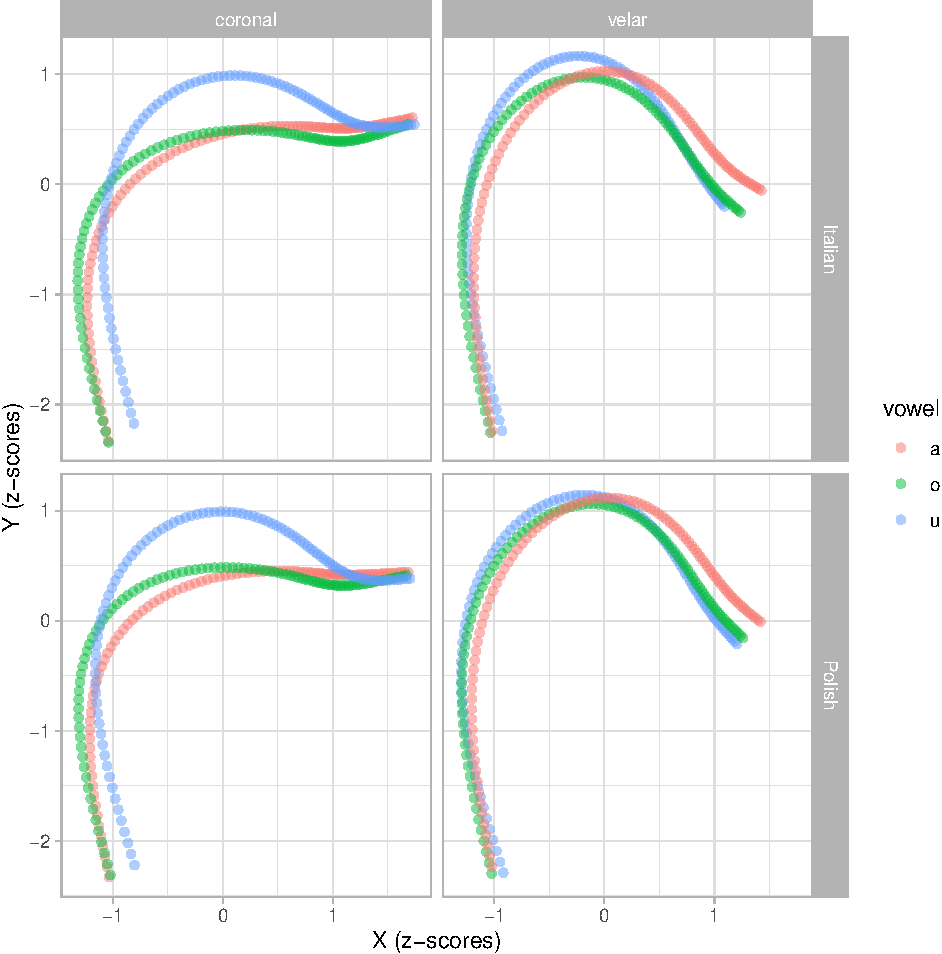
\includegraphics[keepaspectratio]{index_files/figure-pdf/fig-voff-pred-1.pdf}}

}

\end{figure}%

\phantomsection\label{cell-fig-voff-ci}
\begin{figure}[H]

\caption{\label{fig-voff-ci}Predicted tongue contours based on a
multivariate GAM, with 95\% Confidence Intervals.}

\centering{

\pandocbounded{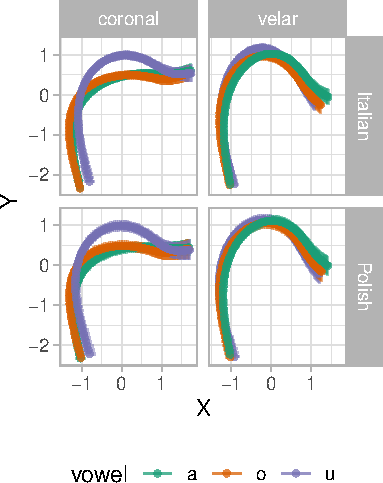
\includegraphics[keepaspectratio]{index_files/figure-pdf/fig-voff-ci-1.pdf}}

}

\end{figure}%

Figure~\ref{fig-voff-ci} strongly suggests greater VC coarticulation on
the C closure in coronal that in velar contexts. Moreover, the vowels
/a, o/ have a similar coarticulatory effect on the tongue contour. With
velar consonants, we observe less coarticulation from the preceding
vowel (an possible explanation of this is given at the end of
Section~\ref{sec-fpca-vc}.

\subsection{Emphaticness}\label{sec-gam-emphaticness}

The second case study is about consonant ``emphaticness'' in Lebanese
Arabic. The data is from Sakr (\citeproc{ref-sakr2025}{2025}). Lebanese
Arabic is a variety of Arabic primarily spoken in Lebanon, where it is
in constant contact with a number of Indo-European languages (primarily
English and French, as vectors of education and business, see eg.
\citeproc{ref-shaaban1999}{Shaaban \& Ghaith, 1999}), as well as the
written standard form of Arabic known as Modern Standard Arabic (MSA).
The relationship between Lebanese Arabic (LA) and MSA in Lebanon is one
of diglossia (see eg. \citeproc{ref-lian2022}{Lian, 2022}), where LA is
spoken in most contexts, but not written, and MSA is the written
variety, and therefore also primarily used for legal and official
purposes.

Emphasis is a phonologically contrastive feature of Semitic languages.
In most varieties of Arabic, it is usually reported to be realised as
pharyngealisation (\citeproc{ref-al-tamimi2017}{J. Al-Tamimi, 2017};
\citeproc{ref-sakr2023}{Sakr, 2023}; \citeproc{ref-watson2002}{Watson,
2002}; \citeproc{ref-zeroual2011}{Zeroual et al., 2011}) with some
variation depending on phonological context
(\citeproc{ref-al-tamimi2011}{F. Al-Tamimi \& Heselwood, 2011};
\citeproc{ref-sakr2025}{Sakr, 2025}) or on sociolinguistic factors
(\citeproc{ref-khattab2006}{Khattab et al., 2006}). Older sources
instead report the secondary place of articulation as being the velum
(\citeproc{ref-nasr1959}{Nasr, 1959}; see eg.
\citeproc{ref-obrecht1968}{Obrecht, 1968}) or the uvula (see eg.
\citeproc{ref-bin-muqbil2006}{Bin-Muqbil, 2006};
\citeproc{ref-ghazeli1977}{Ghazeli, 1977};
\citeproc{ref-zawaydeh1999}{Zawaydeh, 1999}). Whatever the specifics of
this secondary place of articulation, the literature additionally
suggests the occurrence of a loss of emphasis in Lebanese, or more
generally Levantine or Western dialects of Arabic, likely as a result of
the contact with the Indo-European languages mentioned above
(\citeproc{ref-alorifi2008}{Alorifi, 2008};
\citeproc{ref-elhija2012}{Elhij'a, 2012};
\citeproc{ref-el-khaissi2015}{El-Khaissi, 2015}; see among others
\citeproc{ref-sullivan2017}{Sullivan, 2017}).

It is against this background, and as part of efforts to document the
precise place of secondary articulation of emphasis in Lebanese Arabic,
as well as to document whether or not emphasis has, indeed, been lost in
the variety, that the data used here (from \citeproc{ref-sakr2025}{Sakr,
2025}) was collected. It consists of UTI recordings, by 5 participants,
of CVb stimuli. The onset was either an emphatic or an unemphatic
(`plain'), voiced or voiceless, alveolar, plosive or fricative /t, ṭ, d,
ḍ, s, ṣ, z, ẓ/; when talking about a plain/emphatic pair, we denote them
/T, D, S, Z/. The nucleus was one of five vowel qualities (see
\citeproc{ref-sakr2019}{Sakr, 2019}) present in Lebanese, which we will
denote with /A, E, I, O, U/ to signal that these are neither to be taken
as phonemes or exact phonetic realisations. The coda was the voiced
bilabial plosive /b/. Each recording consisted of four stimuli in
randomized order, covering forty syllables, in five repetitions; for a
total of 1000 recordings. The subset of the data used here is from 35ms
before consonant offset, defined as the burst for the plosives and as
the end of the frication noise for the fricatives.

Since the procedure to fit and plot MGAMs is the same as the one
presented in Section~\ref{sec-gam-vc-coart}, we won't be showing the
code in this section, but readers can find the code in the
\href{index.qmd}{Article Notebook}.

Figure~\ref{fig-emph-ci} shows the predicted tongue contours of emphatic
and plain consonants, split by following vowel. First, the following
vowel exercises an appreciable amount of coarticulation on the preceding
consonant. The vowel-induced coarticulation seem to be modulating how
the emphatic vs plain distinction is implemented (or not): in the
context of the vowels /A, O, U/, emphatic consonants are produced with a
retracted body and root, indicating pharyngealisation. On the other
hand, in the context of the front vowels /E, I/, there is visibly less
distinction between emphatic and plain consonants, which is virtually
absent in /E/. However, when plotting the predictions for the different
vocalic contexts and different speakers, the picture becomes more
complex.

\phantomsection\label{cell-fig-emph-ci}
\begin{figure}[H]

\caption{\label{fig-emph-ci}Predicted tongue contours with 95\% CIs from
an MGAM of Lebanese Arabic emphatic and plain coronal consonants.}

\centering{

\pandocbounded{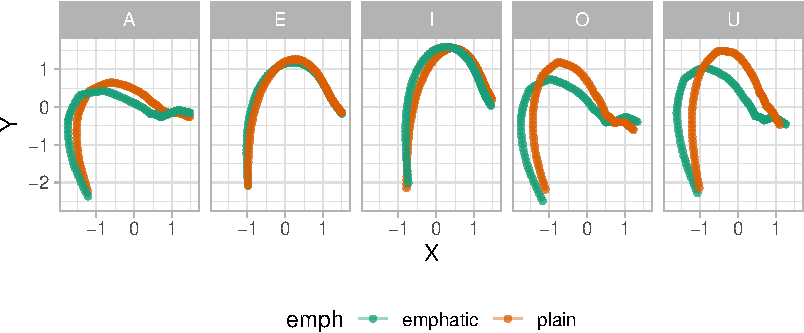
\includegraphics[keepaspectratio]{index_files/figure-pdf/fig-emph-ci-1.pdf}}

}

\end{figure}%

In Figure~\ref{fig-emph-part}, predictions have been calculated for
individual speakers (see Article Notebook online, linked above, for the
code). First, there is a good deal of individual variation: some
speakers show a clear differentiation of the tongue shape in emphatic
and plain consonants, while in other speakers the difference is less
obvious. FAK produced emphatic and plain consonants with virtually the
same tongue shape. Just to pick another example, BAR
uvularised/velarised rather than pharyngealised the emphatic consonants
followed by /I/, while BAY pharyngealised them. Plotting predictions of
individual speakers can reveal idiosyncratic patterns which are not
visible when plotting overall predictions.

\phantomsection\label{cell-fig-emph-part}
\begin{figure}[H]

\caption{\label{fig-emph-part}Predicted tongue contours with 95\% CIs
from an MGAM of Lebanese Arabic emphatic and plain coronal consonants
split by speaker.}

\centering{

\pandocbounded{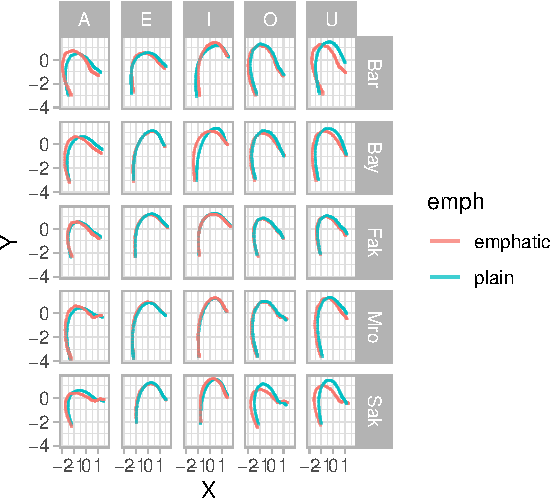
\includegraphics[keepaspectratio]{index_files/figure-pdf/fig-emph-part-1.pdf}}

}

\end{figure}%

\section{Multivariate Functional Principal Component
Analysis}\label{sec-fpca}

Principal Component Analysis (PCA) is a dimensionality reduction
technique. For an introduction to PCA we recommend Kassambara
(\citeproc{ref-kassambara2017a}{2017}). Functional PCA (FPCA) is an
extension of PCA: while classical PCA works by finding common variance
in a set of variables (and by reducing the variables to Principal
Components that explain that common variance), FPCA is a PCA applied to
a functional representation of varying numerical variables
(\citeproc{ref-gubian2019}{Gubian, Harrington, et al., 2019};
\citeproc{ref-gubian2019a}{Gubian, Pastätter, et al., 2019};
\citeproc{ref-gubian2024}{Gubian, 2024}): a typical example is
time-series data, with a variable changing over time. The trajectory of
the time-varying variable is encoded into a function with a set of
coefficients and the values of those coefficients are submitted to PCA.
When more than one time-varying variable is needed, this is where
Multivariate FPCA (MFPCA) come in (\citeproc{ref-gubian2024}{Gubian,
2024}).

MFPCA is an FPCA applied to two or more varying variables. Note that the
variable does not have to be \emph{time}-varying. The variation can be
on any linear variable: in the case of DLC-tracked UTI data, the
variation happens along the knot number. Look back at
Figure~\ref{fig-tongue-xy}: the two varying variables are the X and Y
coordinates, which are varying along the DLC knots. As with MGAMs, it is
these two varying trajectories that are submitted to MFPCA.

\subsection{VC coarticulation}\label{sec-fpca-vc}

We will apply Multivariate Functional Principal Component Analysis
(MFPCA) to the data introduced in Section~\ref{sec-gam-vc-coart}. The
following code has been adapted from Gubian
(\citeproc{ref-gubian2024}{2024}). The packages below are needed to run
MFPCA (except landmarkregUtils, they are available on CRAN).

\begin{Shaded}
\begin{Highlighting}[]
\FunctionTok{library}\NormalTok{(fda)}
\end{Highlighting}
\end{Shaded}

\begin{Shaded}
\begin{Highlighting}[]
\FunctionTok{library}\NormalTok{(funData)}
\end{Highlighting}
\end{Shaded}

\begin{Shaded}
\begin{Highlighting}[]
\FunctionTok{library}\NormalTok{(MFPCA)}
\CommentTok{\# install.packages("remotes")}
\CommentTok{\# remotes::install\_github("uasolo/landmarkregUtils")}
\FunctionTok{library}\NormalTok{(landmarkregUtils)}
\end{Highlighting}
\end{Shaded}

The format required to work through MFPCA is a ``long'' format with one
column containing the coordinate labels (\emph{x} or \emph{y}
coordinate) and another with the coordinate values. We can easily pivot
the data with \texttt{pivot\_longer()}. Note that we are using the
\emph{z}-scored coordinate values (\texttt{X\_z} and \texttt{Y\_z}). If
you are not unsure about what the code in this section, it is always
useful to inspect intermediate and final output in the pipe chains to
familiarise yourself with the format of the input and resulting data.

\begin{Shaded}
\begin{Highlighting}[]
\NormalTok{dlc\_voff\_long }\OtherTok{\textless{}{-}}\NormalTok{ dlc\_voff\_f }\SpecialCharTok{|\textgreater{}} 
  \CommentTok{\# Select relevant columns}
\NormalTok{  dplyr}\SpecialCharTok{::}\FunctionTok{select}\NormalTok{(X\_z, Y\_z, frame\_id, knot, vowel, c2\_place, language, speaker) }\SpecialCharTok{|\textgreater{}} 
  \CommentTok{\# Pivot data to longer format. Saves coordinate labels to column \textasciigrave{}dim\textasciigrave{}}
  \FunctionTok{pivot\_longer}\NormalTok{(}\FunctionTok{c}\NormalTok{(X\_z, Y\_z), }\AttributeTok{names\_to =} \StringTok{"dim"}\NormalTok{)}
\end{Highlighting}
\end{Shaded}

In the second step, we create a \texttt{multiFunData} object: this is a
special type of list object, with the observations of the two
coordinates (\texttt{X\_z} and \texttt{Y\_z}) as two matrices of
dimension \(N \cdot 11\), where \(N\) is the number of tongue contours
and \(11\) is for the 11 knots returned by DLC. Three columns in the
data are used to create the \texttt{multiFunData} object: one column
with the id of each contour (in our data, \texttt{frame\_id}), a time or
series column (\texttt{knot}) and the column with the coordinate values
(\texttt{value}).

\begin{Shaded}
\begin{Highlighting}[]
\NormalTok{curves\_fun\_2d }\OtherTok{\textless{}{-}} \FunctionTok{lapply}\NormalTok{(}
  \FunctionTok{c}\NormalTok{(}\StringTok{"X\_z"}\NormalTok{, }\StringTok{"Y\_z"}\NormalTok{),}
  \ControlFlowTok{function}\NormalTok{(y) \{}
    \FunctionTok{long2irregFunData}\NormalTok{(}
\NormalTok{      dlc\_voff\_long }\SpecialCharTok{|\textgreater{}} \FunctionTok{filter}\NormalTok{(dim }\SpecialCharTok{==}\NormalTok{ \{\{y\}\}),}
      \CommentTok{\# Tongue contour ID}
      \AttributeTok{id =} \StringTok{"frame\_id"}\NormalTok{,}
      \CommentTok{\# Knot column}
      \AttributeTok{time =} \StringTok{"knot"}\NormalTok{,}
      \CommentTok{\# X/Y coordinate values}
      \AttributeTok{value =} \StringTok{"value"}
\NormalTok{    ) }\SpecialCharTok{|\textgreater{}} 
    \FunctionTok{as.funData}\NormalTok{()}
\NormalTok{  \}}
\NormalTok{) }\SpecialCharTok{|\textgreater{}} 
  \FunctionTok{multiFunData}\NormalTok{()}
\end{Highlighting}
\end{Shaded}

Once we have our \texttt{multiFunData} object, we can use the
\texttt{MFPCA()} function to compute an MFPCA. In this tutorial we will
compute the first two PCs, but you can compute up to \(K-1\) PCs where
\(K\) is the number of DLC knots in the data.

\begin{Shaded}
\begin{Highlighting}[]
\CommentTok{\# Number of PC to compute}
\NormalTok{n\_pc }\OtherTok{\textless{}{-}} \DecValTok{2}

\CommentTok{\# Compute MFPCA}
\NormalTok{mfpca }\OtherTok{\textless{}{-}} \FunctionTok{MFPCA}\NormalTok{(}
\NormalTok{  curves\_fun\_2d,}
  \AttributeTok{M =}\NormalTok{ n\_pc,}
  \AttributeTok{uniExpansions =} \FunctionTok{list}\NormalTok{(}\FunctionTok{list}\NormalTok{(}\AttributeTok{type =} \StringTok{"uFPCA"}\NormalTok{), }\FunctionTok{list}\NormalTok{(}\AttributeTok{type =} \StringTok{"uFPCA"}\NormalTok{))}
\NormalTok{)}
\end{Highlighting}
\end{Shaded}

We can quickly calculate the proportion of explained variance of each PC
with the following code. Since we have calculated only two PCs, PC1 and
PC2 together explain 100\% of the variance in our data. For each PC that
is calculated, the higher the variance explained, the better the
variance patterns in the data are captured.

\begin{Shaded}
\begin{Highlighting}[]
\CommentTok{\# Proportion of explained variance}
\NormalTok{mfpca}\SpecialCharTok{$}\NormalTok{values  }\SpecialCharTok{/} \FunctionTok{sum}\NormalTok{(mfpca}\SpecialCharTok{$}\NormalTok{values)}
\end{Highlighting}
\end{Shaded}

\begin{verbatim}
[1] 0.7108713 0.2891287
\end{verbatim}

The best way to assess the effect of the PC scores on the shape of the
tongue contours is to plot the predicted tongue contours based on a set
of representative PC scores. In order to be able to plot the predicted
contours, we need to calculate them from the MFPCA object. Gubian
suggests plotting predicted curves at score intervals based on fractions
of the scores standard deviation. This is what the following code does.

\begin{Shaded}
\begin{Highlighting}[]
\CommentTok{\# Get the PC score SD}
\NormalTok{sd\_fun }\OtherTok{\textless{}{-}} \FunctionTok{sqrt}\NormalTok{(mfpca}\SpecialCharTok{$}\NormalTok{values)}

\CommentTok{\# PC curves to be plotted}
\NormalTok{pc\_curves }\OtherTok{\textless{}{-}} \FunctionTok{expand\_grid}\NormalTok{(}
  \AttributeTok{PC =} \DecValTok{1}\SpecialCharTok{:}\NormalTok{n\_pc,}
  \AttributeTok{dim =} \DecValTok{1}\SpecialCharTok{:}\DecValTok{2}\NormalTok{,}
  \CommentTok{\# Set the SD fraction, from {-}1 SD to +1 SD, with increments by 0.25}
  \AttributeTok{sd\_frac =} \FunctionTok{seq}\NormalTok{(}\SpecialCharTok{{-}}\DecValTok{1}\NormalTok{, }\DecValTok{1}\NormalTok{, }\AttributeTok{by =} \FloatTok{0.25}\NormalTok{)}
\NormalTok{) }\SpecialCharTok{|\textgreater{}}
  \FunctionTok{group\_by}\NormalTok{(PC, dim, sd\_frac) }\SpecialCharTok{|\textgreater{}}
  \CommentTok{\# We can now calculate the predicted contour with funData2long1().}
  \CommentTok{\# reframe() is needed because the funData2long1() function returns a data frame}
  \CommentTok{\# the has more rows than the original.}
  \FunctionTok{reframe}\NormalTok{(}
    \FunctionTok{funData2long1}\NormalTok{(}
\NormalTok{      mfpca}\SpecialCharTok{$}\NormalTok{meanFunction[[dim]] }\SpecialCharTok{+}
\NormalTok{        sd\_frac }\SpecialCharTok{*}\NormalTok{ sd\_fun[PC] }\SpecialCharTok{*}\NormalTok{ mfpca}\SpecialCharTok{$}\NormalTok{functions[[dim]][PC],}
      \AttributeTok{time =} \StringTok{"knot"}\NormalTok{, }\AttributeTok{value =} \StringTok{"value"}
\NormalTok{    )}
\NormalTok{  ) }\SpecialCharTok{|\textgreater{}} 
  \CommentTok{\# We relabel the dimensions}
  \FunctionTok{mutate}\NormalTok{(}
    \AttributeTok{dim =} \FunctionTok{factor}\NormalTok{(dim, }\AttributeTok{levels =} \FunctionTok{c}\NormalTok{(}\DecValTok{2}\NormalTok{, }\DecValTok{1}\NormalTok{), }\AttributeTok{labels =} \FunctionTok{c}\NormalTok{(}\StringTok{\textquotesingle{}Y\_z\textquotesingle{}}\NormalTok{, }\StringTok{\textquotesingle{}X\_z\textquotesingle{}}\NormalTok{))}
\NormalTok{  )}
\end{Highlighting}
\end{Shaded}

The created data frame \texttt{pc\_curves} has the predicted values of
the X and Y coordinates \emph{along the knots}. This is the same
structure as Figure~\ref{fig-tongue-xy}, with the knot number on the
\emph{x}-axis and the coordinates on the \emph{y}-axis. Of course, what
we are after is the X/Y plot of the tongue contours, rather than the
knot/coordinate plot as needed to fit an MFPCA. For the sake of clarity,
we first plot the predicted curves for X and Y separately.
Figure~\ref{fig-pc-curves} shows these. The plot is composed of four
panels: the top two are the predicted curves along knot number for the Y
coordinates (based on PC1 in the left panel and PC2 in the right panel).
Interpreting the effect of the PCs on the X and Y coordinates separately
allows one to observe vertical (Y coordinate) and horizontal (X
coordinate) differences in tongue position independently. However, note
that the vectors of muscle contractions in the tongue are not simply
along a vertical/horizontal axis (\citeproc{ref-honda1996}{Honda, 1996};
\citeproc{ref-wrench2024}{Wrench, 2024}). Looking at a full tongue
contour (in an X/Y coordinates plot) will generally prove to be more
straightforward.

\phantomsection\label{cell-fig-pc-curves}
\begin{figure}[H]

\caption{\label{fig-pc-curves}Predicted curves along knot number for X
and Y coordinates, as obtained from an MFPCA.}

\centering{

\pandocbounded{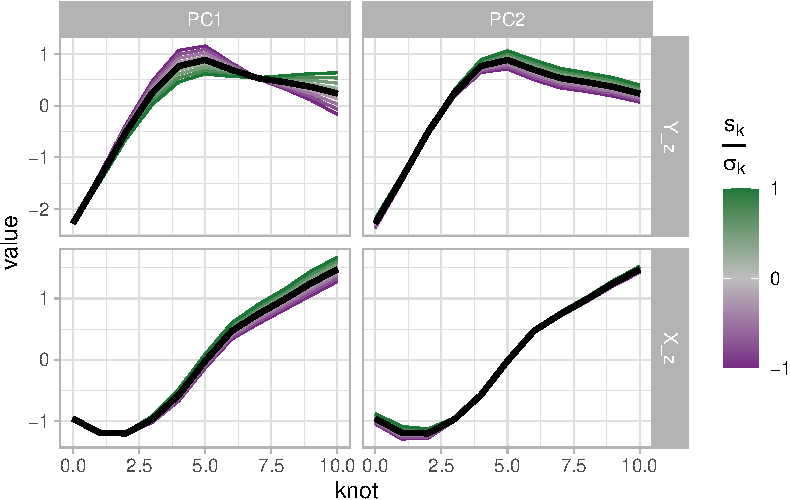
\includegraphics[keepaspectratio]{index_files/figure-pdf/fig-pc-curves-1.pdf}}

}

\end{figure}%

In order to plot tongue contours in the X/Y coordinate system, we simply
need to pivot the data to a wider format.

\begin{Shaded}
\begin{Highlighting}[]
\NormalTok{pc\_curves\_wide }\OtherTok{\textless{}{-}}\NormalTok{ pc\_curves }\SpecialCharTok{|\textgreater{}} 
  \FunctionTok{pivot\_wider}\NormalTok{(}\AttributeTok{names\_from =}\NormalTok{ dim)}
\end{Highlighting}
\end{Shaded}

Figure~\ref{fig-contours} plots the predicted contours based on the the
PC scores (specifically, fractions of the standard deviation of the PC
scores). The \emph{x} and \emph{y}-axes correspond to the X and Y
coordinates of the tongue contour, with the effect of PC1 in the left
panel and the effect of PC2 in the right panel. A higher PC1 score
(green lines in the left panel) suggest a lowering of the tongue
body/dorsum and raising of the tongue tip. Since the data contains velar
and coronal consonants, we take this to be capturing the velar/coronal
place of articulation effect. A higher PC2 score (green lines in the
right panel) corresponds to an overall higher tongue position.
Considering that the back/central vowels /a, o, u/ are included in this
data set, we take PC2 to be related with the effect of vowel on the
tongue shape at closure onset.

\phantomsection\label{cell-fig-contours}
\begin{figure}[H]

\caption{\label{fig-contours}Predicted tongue contours as obtained from
an MFPCA.}

\centering{

\pandocbounded{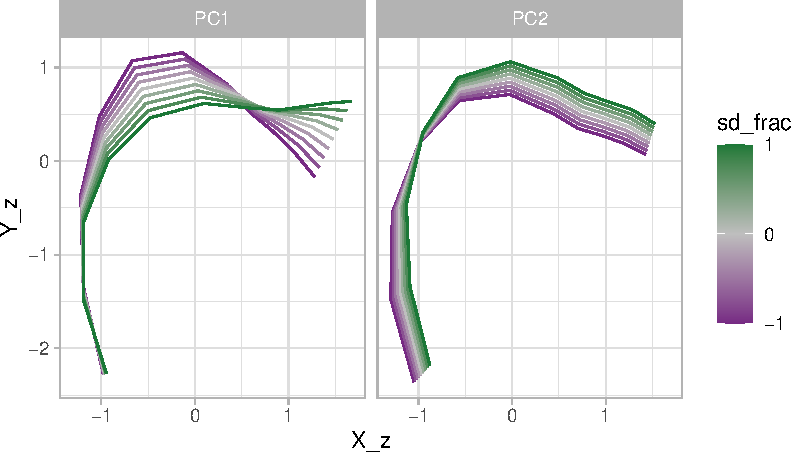
\includegraphics[keepaspectratio]{index_files/figure-pdf/fig-contours-1.pdf}}

}

\end{figure}%

Given the patterns in Figure~\ref{fig-contours}, we can expect to see
differences in PC2 scores based on the vowel if there is VC
coarticulation. We can obtain the PC scores of each observation in the
data with the following code.

\begin{Shaded}
\begin{Highlighting}[]
\NormalTok{pc\_scores }\OtherTok{\textless{}{-}}\NormalTok{ mfpca}\SpecialCharTok{$}\NormalTok{scores }\SpecialCharTok{|\textgreater{}}
  \StringTok{\textasciigrave{}}\AttributeTok{colnames\textless{}{-}}\StringTok{\textasciigrave{}}\NormalTok{(}\FunctionTok{paste0}\NormalTok{(}\StringTok{"PC"}\NormalTok{, }\DecValTok{1}\SpecialCharTok{:}\NormalTok{n\_pc)) }\SpecialCharTok{|\textgreater{}}
  \FunctionTok{as\_tibble}\NormalTok{() }\SpecialCharTok{|\textgreater{}}
  \FunctionTok{bind\_cols}\NormalTok{(dlc\_voff\_long }\SpecialCharTok{|\textgreater{}} \FunctionTok{distinct}\NormalTok{(frame\_id, vowel, c2\_place, language))}
\end{Highlighting}
\end{Shaded}

Figure~\ref{fig-pc-scores} plots PC scores by language (rows), consonant
place (columns) and vowel (colour). Both in Italian and Polish, we can
observe a clear coarticulatory effect of /u/ on the production of
coronal stops (and perhaps minor differences in /a/ vs /o/). On the
other hand, the effect of vowel in velar stops seems to be minimal,
again in both languages. This is not entirely surprising, since while
coronal stops allow for adjustments of (and coarticulatory effect on)
the tongue body, velar stops do not since it is precisely the tongue
body/dorsum that is raised to produce the velar closure.

\phantomsection\label{cell-fig-pc-scores}
\begin{figure}[H]

\caption{\label{fig-pc-scores}PC1/PC2 scores by language, consonant
place of articulation and vowel.}

\centering{

\pandocbounded{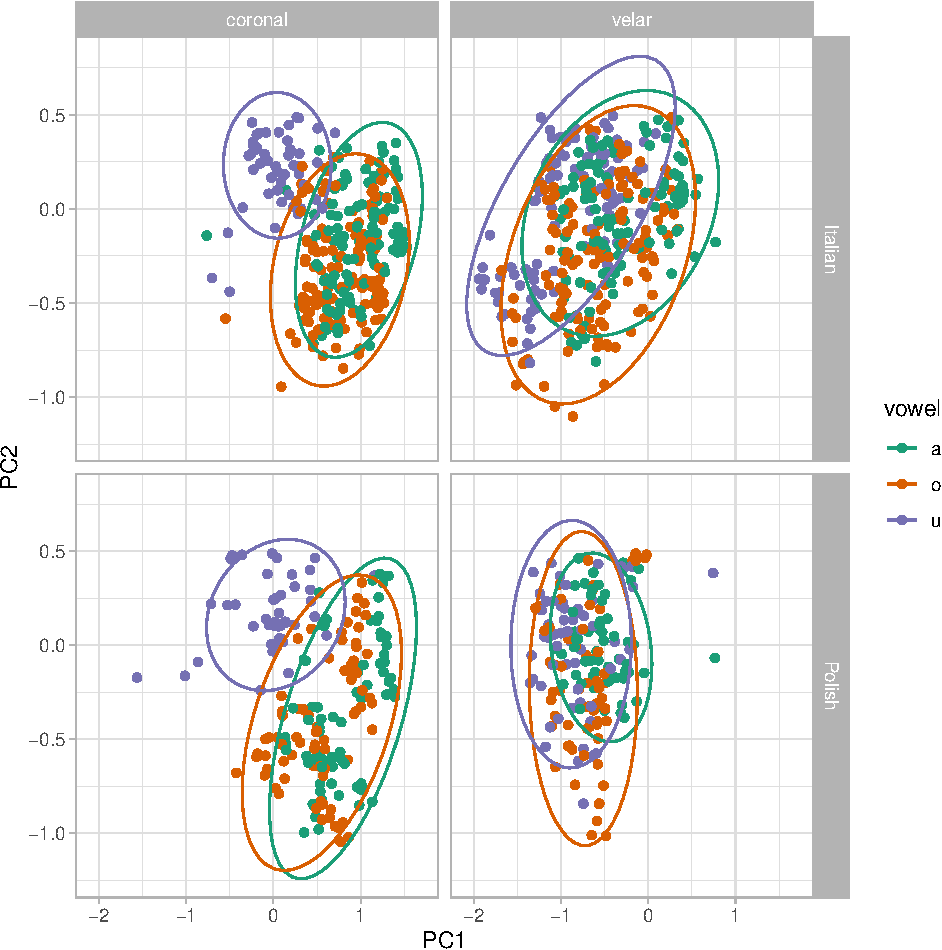
\includegraphics[keepaspectratio]{index_files/figure-pdf/fig-pc-scores-1.pdf}}

}

\end{figure}%

Once one has established which patterns each PC is capturing, PC scores
can be submitted to further statistical modelling, like for example
regression models where the PC scores are outcome variables and several
predictors are included to assess possible differences in PC scores.

\subsection{Emphaticness}\label{emphaticness}

In this section we will run an MFPCA analysis on the Lebanese Arabic
data. Since the procedure is the same as in the previous section, the
code will not be shown here, but can be viewed in the
\href{index.qmd}{Article Notebook}.

Figure~\ref{fig-emph-curves-wide} illustrates the reconstructed tongue
contours (taken from 35 ms before the CV boundary) in Lebanese Arabic,
based on the MFPCA. PC1 captures the low-back/high-front diagonal
movement. PC2, on the other hand, seems to be restricted to high/low
movement at the back of the oral cavity. Emphatic consonants, if
produced with a constricted pharynx (i.e.~pharyngealised), should have a
lower PC1. If on the other hand they are produced with a raised tongue
dorsum (i.e.~uvularised/velarised), they should have a lower PC2 (lower
PC scores are in purple in Figure~\ref{fig-emph-curves-wide}).

\phantomsection\label{cell-fig-emph-curves-wide}
\begin{figure}[H]

\caption{\label{fig-emph-curves-wide}Predicted tongue contours of
Lebanese Arabic coronal consonants as obtained from an MFPCA.}

\centering{

\pandocbounded{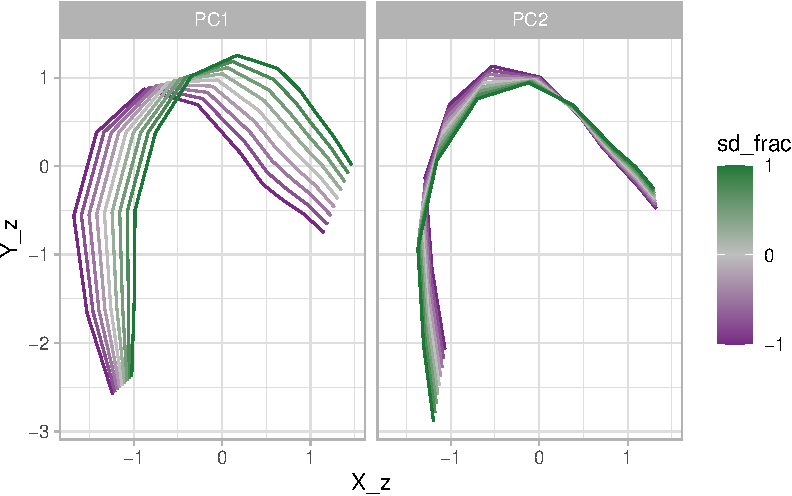
\includegraphics[keepaspectratio]{index_files/figure-pdf/fig-emph-curves-wide-1.pdf}}

}

\end{figure}%

Figure~\ref{fig-emph-speakers} plots the PC scores for each vowel,
emphaticness and speaker combination. Points are coloured based on
emphaticness: emphatic in green and plain in orange. This figure
illustrates well how the PC scores can capture individual variation:
some speakers show clear separation of emphatic and plain tokens, while
others do not. In most cases, PC1 is doing the heavy lifting of
distinguishing emphatic and plain: recall that PC1 captures the
front-high/back-low diagonal; a low PC1 indicates tongue dorsum and root
backing, in other words pharyngealisation. Indeed, PC1 tends to be lower
in emphatic tokens in several speakers, like Bar, Bay, Mro and Sak,
especially with the vowels /A, O, U/. On the other hand, Bar's emphatic
and plain tokens for vowels /E, I/ do not show a PC1 difference, but
rather a PC2 difference: PC2 captures tongue dorsum/body raising, hence
indicating velarisation. It is possible that in Bar's productions of
emphatic consonants followed by /E, I/ the distinction with plain is
produced by uvularisation/velarisation, compared to the
pharyngealisation of emphatic consonants followed by /A, O, U/.
Uvularisation/velarisation, rather than pharyngealisation, in the /E, I/
contexts makes sense given that the tongue root has to be front in the
production of those vowels (see Sakr (\citeproc{ref-sakr2025}{2025}),
Section 6.4 for more details).

\phantomsection\label{cell-fig-emph-speakers}
\begin{figure}[H]

\caption{\label{fig-emph-speakers}PC1 and PC2 scores by vowel, consonant
type and speaker.}

\centering{

\pandocbounded{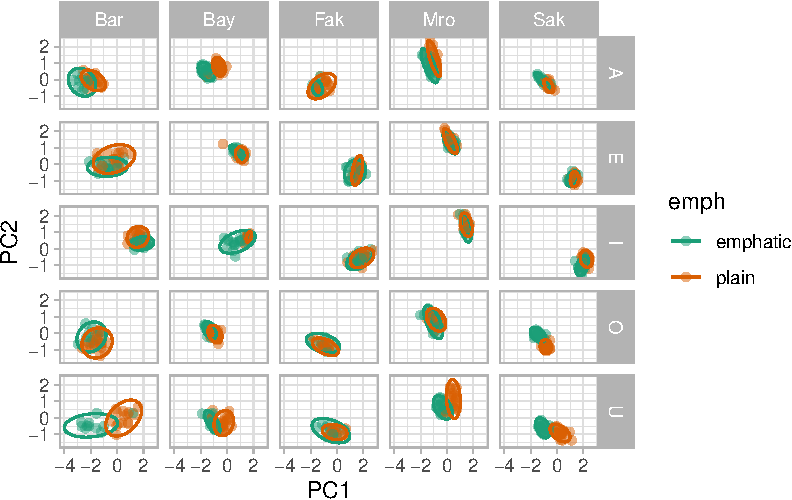
\includegraphics[keepaspectratio]{index_files/figure-pdf/fig-emph-speakers-1.pdf}}

}

\end{figure}%

Figure~\ref{fig-emph-pc1} and Figure~\ref{fig-emph-pc2} illustrate one
way to plot the PC scores individually for PC1 and PC2. We won't include
here a full description of the plots, since they should be
self-explanatory, but we flag to the reader that these type of plots can
be helpful in illustrating specific patterns in PC1 or PC2.

\phantomsection\label{cell-fig-emph-pc1}
\begin{figure}[H]

\caption{\label{fig-emph-pc1}PC1 scores of emphatic and plain consonants
by speaker and vowel.}

\centering{

\pandocbounded{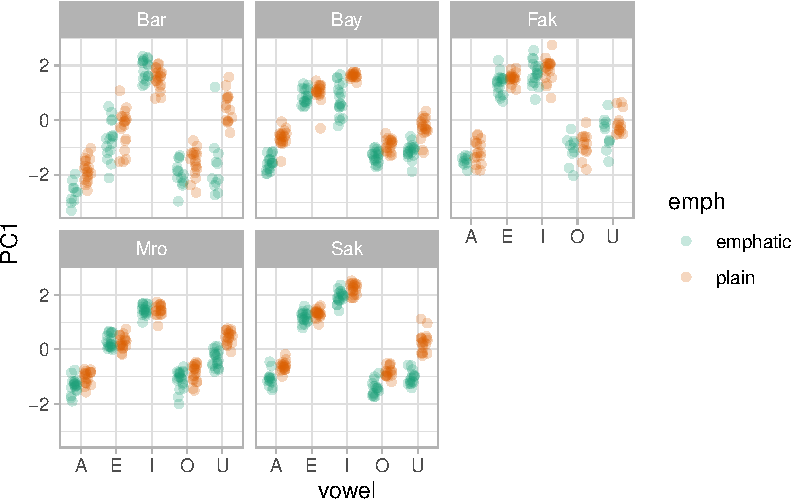
\includegraphics[keepaspectratio]{index_files/figure-pdf/fig-emph-pc1-1.pdf}}

}

\end{figure}%

\phantomsection\label{cell-fig-emph-pc2}
\begin{figure}[H]

\caption{\label{fig-emph-pc2}PC2 scores of emphatic and plain consonants
by speaker and vowel.}

\centering{

\pandocbounded{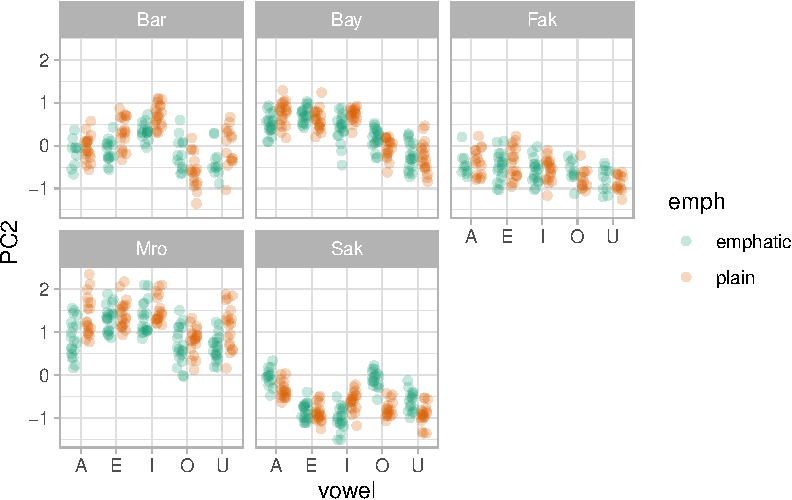
\includegraphics[keepaspectratio]{index_files/figure-pdf/fig-emph-pc2-1.pdf}}

}

\end{figure}%

Finally, it will usually be helpful to reconstruct the predicted tongue
contours of specific context. For example, we might be interested in
showing the average tongue contours for emphatic and plain consonant
followed by each of the five vowels in the data. This is shown in
Figure~\ref{fig-vow-emph}. In order to obtain the reconstructed
contours, we first need to calculate mean PC scores for each vowel. This
can be done through the following code. We recommend to inspect the
\texttt{pc\_scores\_mean} object.

\begin{Shaded}
\begin{Highlighting}[]
\NormalTok{pc\_scores\_mean }\OtherTok{\textless{}{-}}\NormalTok{ pc\_scores }\SpecialCharTok{|\textgreater{}}
  \CommentTok{\# Group by variables based on which we want to obtain mean values.}
  \FunctionTok{group\_by}\NormalTok{(vowel, emph) }\SpecialCharTok{|\textgreater{}} 
  \CommentTok{\# Sumarise data to obtain means}
  \FunctionTok{summarise}\NormalTok{(}
    \AttributeTok{PC1 =} \FunctionTok{mean}\NormalTok{(PC1),}
    \AttributeTok{PC2 =} \FunctionTok{mean}\NormalTok{(PC2),}
    \AttributeTok{.groups =} \StringTok{"drop"}
\NormalTok{  ) }\SpecialCharTok{|\textgreater{}} 
  \CommentTok{\# Add "dimensions", i.e. X and Y coordinates}
  \FunctionTok{mutate}\NormalTok{(}
    \AttributeTok{dim =} \FunctionTok{list}\NormalTok{(}\FunctionTok{c}\NormalTok{(}\DecValTok{1}\NormalTok{, }\DecValTok{2}\NormalTok{))}
\NormalTok{  ) }\SpecialCharTok{|\textgreater{}} 
  \CommentTok{\# Unnes the dim column}
  \FunctionTok{unnest}\NormalTok{(dim)}
\end{Highlighting}
\end{Shaded}

The following code calculates the reconstructed tongue contours based on
both PC1 and PC2. One could also calculate the reconstructed contours at
factions of the standard deviation of the scores if one wished so, like
it was done above.

\begin{Shaded}
\begin{Highlighting}[]
\NormalTok{pc\_curves\_2 }\OtherTok{\textless{}{-}}\NormalTok{ pc\_scores\_mean }\SpecialCharTok{|\textgreater{}} 
  \FunctionTok{group\_by}\NormalTok{(dim, vowel, emph) }\SpecialCharTok{|\textgreater{}}
  \CommentTok{\# We can now calculate the predicted contour with funData2long1().}
  \CommentTok{\# reframe() is needed because the funData2long1() function returns a data frame}
  \CommentTok{\# the has more rows than the original.}
  \FunctionTok{reframe}\NormalTok{(}
    \FunctionTok{funData2long1}\NormalTok{(}
\NormalTok{      mfpca}\SpecialCharTok{$}\NormalTok{meanFunction[[dim]] }\SpecialCharTok{+}
        \CommentTok{\# We add PC1}
\NormalTok{        PC1 }\SpecialCharTok{*}\NormalTok{ mfpca}\SpecialCharTok{$}\NormalTok{functions[[dim]][}\DecValTok{1}\NormalTok{] }\SpecialCharTok{+}
        \CommentTok{\# and we add PC2 as well}
\NormalTok{        PC2 }\SpecialCharTok{*}\NormalTok{ mfpca}\SpecialCharTok{$}\NormalTok{functions[[dim]][}\DecValTok{2}\NormalTok{],}
      \AttributeTok{time =} \StringTok{"knot"}\NormalTok{, }\AttributeTok{value =} \StringTok{"value"}
\NormalTok{    )}
\NormalTok{  ) }\SpecialCharTok{|\textgreater{}} 
  \CommentTok{\# We relabel the dimensions}
  \FunctionTok{mutate}\NormalTok{(}
    \AttributeTok{dim =} \FunctionTok{factor}\NormalTok{(dim, }\AttributeTok{levels =} \FunctionTok{c}\NormalTok{(}\DecValTok{2}\NormalTok{,}\DecValTok{1}\NormalTok{), }\AttributeTok{labels =} \FunctionTok{c}\NormalTok{(}\StringTok{\textquotesingle{}Y\_z\textquotesingle{}}\NormalTok{, }\StringTok{\textquotesingle{}X\_z\textquotesingle{}}\NormalTok{))}
\NormalTok{  ) }\SpecialCharTok{|\textgreater{}} 
  \FunctionTok{pivot\_wider}\NormalTok{(}\AttributeTok{names\_from =}\NormalTok{ dim, }\AttributeTok{values\_from =}\NormalTok{ value)}
\end{Highlighting}
\end{Shaded}

Finally, Figure~\ref{fig-vow-emph} plots the reconstructed contours.
Based on this figure, we do find pharyngealisation in emphatic
consonants followed by /A, O, U/ on average, while pharyngealisation is
absent in the context of /E, I/.

\phantomsection\label{cell-fig-vow-emph}
\begin{figure}[H]

\caption{\label{fig-vow-emph}Reconstructed tongue contours based on
PC1/PC2.}

\centering{

\pandocbounded{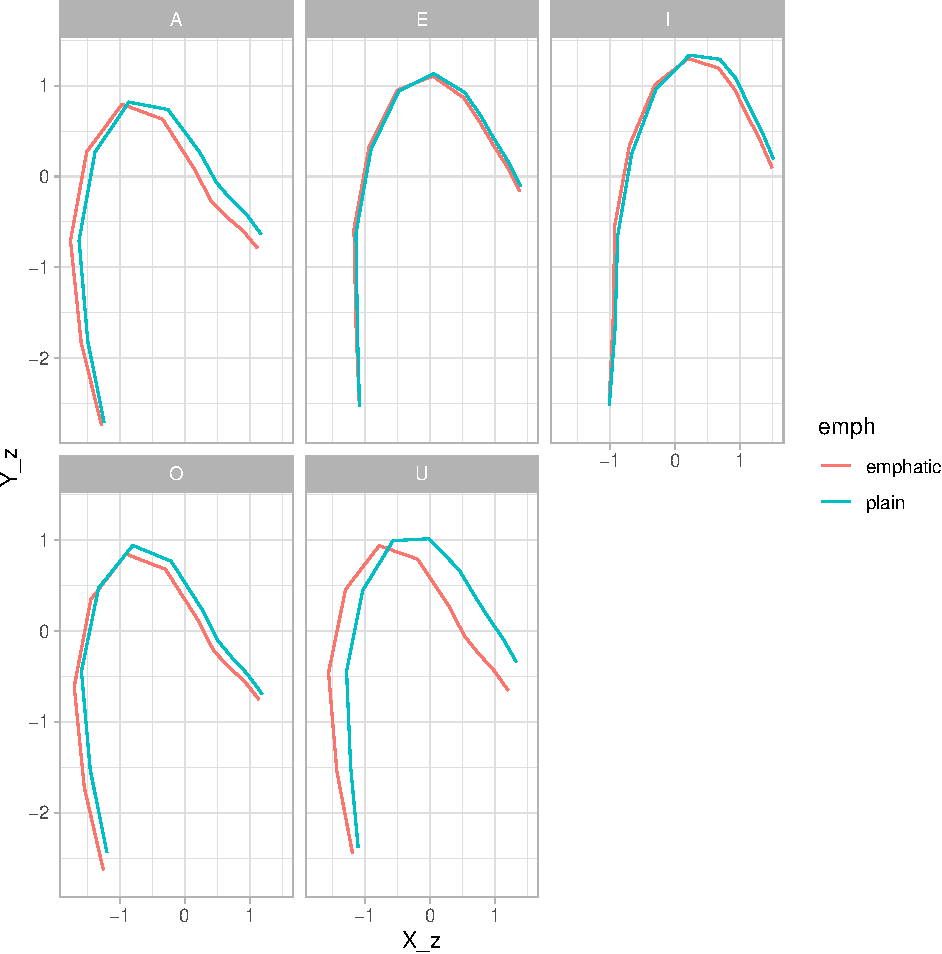
\includegraphics[keepaspectratio]{index_files/figure-pdf/fig-vow-emph-1.pdf}}

}

\end{figure}%

\section{Advantages and disadvantages}\label{sec-procons}

Both Multivariate GAMs and FPCA are a useful way to model DLC-tracked
ultrasound tongue imaging data. However, each possesses advantages and
disadvantages.

Multivariate GAMs can model tongue contours in specific contexts and
combinations thereof, like different vowels, consonant, prosodic
contexts and so on. The rather complex model structure required to fit
multivariate GAMs to tongue data comes at a computational cost and an
interpretative cost. Computationally, multivariate GAMs can take hours
to estimate even the most simple models. Interpretationally, comparing
different tongue contours quantitatively based on the output of a
multivariate GAM is non-trivial, given that the tongue contour is in
fact a curve reconstructed from the smooths of the X and Y coordinates
along knot (in other words, the model does not model tongue contours
directly). Moreover, there is no straightforward way to use traditional
methods to assess (frequentist) statistical significance. From a
practical point of view, a multivariate GAM ends up being a
mathematically complex way of obtaining a sort of average tongue
contour.

Multivariate FPCA, on the other hand, are computationally efficient.
Even with very large data sets, the computation of Principal Components
is relatively quick. Moreover, the obtained PCs can be interpreted
straightforwardly by plotting the effect of changing the PC score on the
reconstructed tongue contour (as we did for example in
Figure~\ref{fig-contours}). One possible disadvantage of multivariate
FPCA is that it is usually not known what type of variation each
obtained PC captures. This is illustrated in the two case studies in
Section~\ref{sec-fpca}. In the VC coarticulation data, PC1 corresponded
to the coronal/velar difference in consonants, while PC2 to the
difference in vowel. In the emphaticness data, PC1 captured the
low-back/high-front diagonal movement, while PC2 to the high/low
movement at the back of the oral cavity. In other words: until one has
run the MFPCA, one cannot know which PC will correspond to which axis of
differences, and whether the PCs will capture relevant differences at
all. It can happen that the variation one is after is so minimal
relative to other, more substantial cases of variation, that it will not
be captured by the MFPCA at all. It is possible that qualitatively
homogeneous data sets might return PCs that have the same or very
similar interpretations, but this has not been systematically tested,
perhaps with the exception of simple PCA run on vowel formant data,
which suggests that the first two PCs capture the two diagonals
(\citeproc{ref-faber1995}{Faber \& Di Paolo, 1995};
\citeproc{ref-hoole1999}{Hoole, 1999};
\citeproc{ref-strycharczuk2021}{Strycharczuk et al., 2021};
\citeproc{ref-strycharczuk2025}{Strycharczuk et al., 2025}), which make
sense in light of the tongue position and shape model expounded by Honda
(\citeproc{ref-honda1996}{1996}).

Another advantage of MFPCA is that, provided that the PCs have captured
relevant characteristics, the PCs can be submitted to further modelling
using regression with the inclusion of relevant predictors (like
different categorical variables of interest). We have not done so in
this tutorial to keep the scope and length of the tutorial manageable,
but both case studies presented in Section~\ref{sec-fpca} are amenable
to such follow-up analysis.

Based on the advantages and disadvantages of each of multivariate GAMs
and FPCA, we suggest to researchers to use MFPCA as the preferred and
default approach to analyse DLC-tracked tongue contour data and to
resort to multivariate GAMs if MFPCA fails to capture relevant
variation.

\section{Conclusions}\label{conclusions}

This tutorial demonstrates two methods for analysing tongue contour data
derived from DeepLabCut: Multivariate Generalised Additive Models
(MGAMs) and Multivariate Functional Principal Component Analysis
(MFPCA). We offer detailed, annotated analyses of two example datasets,
focusing on vowel-to-consonant coarticulation in Italian and Polish, and
emphatic consonants in Lebanese Arabic. All associated materials,
including datasets and code, are accessible through the tutorial's
research compendium at~\url{https://github.com/stefanocoretta/mv_uti}.
In closing, we evaluate the strengths and limitations of each method and
advise adopting MFPCA as the preferred initial modelling strategy for
tongue contour data.

\section*{Disclosure statement}\label{disclosure-statement}
\addcontentsline{toc}{section}{Disclosure statement}

The authors report there are no competing interests to declare.

\section*{\texorpdfstring{\textbf{Data availability
statement}}{Data availability statement}}\label{data-availability-statement}
\addcontentsline{toc}{section}{\textbf{Data availability statement}}

All the materials (inlcuding data and code) are available in the
research compendium of the tutorial at
\url{https://github.com/stefanocoretta/mv_uti}. An online version of the
manuscript is available at
\url{https://stefanocoretta.github.io/mv_uti/}.

\section{References}\label{references}

\phantomsection\label{refs}
\begin{CSLReferences}{1}{0}
\bibitem[\citeproctext]{ref-alorifi2008}
Alorifi, F. S. (2008). \emph{Automatic identification of arabic dialects
using hidden markov models} {[}PhD thesis{]}.

\bibitem[\citeproctext]{ref-al-tamimi2011}
Al-Tamimi, F., \& Heselwood, B. (2011). Nasoendoscopic,
videofluoroscopic and acoustic study of plain and emphatic coronals in
jordanian arabic. \emph{Instrumental Studies in Arabic Phonetics},
\emph{319}, 165191.

\bibitem[\citeproctext]{ref-al-tamimi2017}
Al-Tamimi, J. (2017). Revisiting acoustic correlates of
pharyngealization in jordanian and moroccan arabic: Implications for
formal representations. \emph{Laboratory Phonology: Journal of the
Association for Laboratory Phonology}, \emph{8}(1), 28.
\url{https://doi.org/10.5334/labphon.19}

\bibitem[\citeproctext]{ref-ltd2011}
Articulate Instruments Ldt. (2011). \emph{Articulate assistant advanced
user guide. {Version} 2.16}.

\bibitem[\citeproctext]{ref-bin-muqbil2006}
Bin-Muqbil, M. S. (2006). \emph{Phonetic and phonological aspects of
arabic emphatics and gutturals}. The University of Wisconsin-Madison.

\bibitem[\citeproctext]{ref-chen2011}
Chen, Y., \& Lin, H. (2011). \emph{Analysing tongue shape and movement
in vowel production using SS-ANOVA in ultrasound imaging}. 1721.

\bibitem[\citeproctext]{ref-coretta2019g}
Coretta, S. (n.d.). \emph{Assessing mid-saggital tongue contours in
polar coordinates using generalised additive (mixed) models}.
\url{https://doi.org/10.31219/osf.io/q6vzb}

\bibitem[\citeproctext]{ref-coretta2018f}
Coretta, S. (2018a). \emph{An exploratory study of the voicing effect in
italian and polish {[}data v1.0.0{]}}.
\url{https://doi.org/10.17605/OSF.IO/8ZHKU}

\bibitem[\citeproctext]{ref-coretta2018c}
Coretta, S. (2018b). \emph{Using generalised additive models (GAM) with
polar coordinates for assessing tongue contours}.
\url{https://stefanocoretta.github.io/rticulate/articles/polar-gams.html}

\bibitem[\citeproctext]{ref-coretta2020}
Coretta, S. (2020a). Longer vowel duration correlates with greater
tongue root advancement at vowel offset: Acoustic and articulatory data
from italian and polish. \emph{The Journal of the Acoustical Society of
America}, \emph{147}, 245259. \url{https://doi.org/10.1121/10.0000556}

\bibitem[\citeproctext]{ref-coretta2020b}
Coretta, S. (2020b). \emph{Vowel duration and consonant voicing: A
production study} {[}PhD thesis{]}.

\bibitem[\citeproctext]{ref-davidson2006}
Davidson, L. (2006). Comparing tongue shapes from ultrasound imaging
using smoothing spline analysis of variance. \emph{The Journal of the
Acoustical Society of America}, \emph{120}(1), 407415.
\url{https://doi.org/10.1121/1.2205133}

\bibitem[\citeproctext]{ref-elhija2012}
Elhij'a, D. A. (2012). Facebook Written Levantine Vernacular Languages.
\emph{Levantine Review}, \emph{1}(1), 68105.
\url{https://doaj.org/article/6698290a36c244f783a59ba49617e821}

\bibitem[\citeproctext]{ref-el-khaissi2015}
El-Khaissi, C. (2015). \emph{The romanisation of arabic: A comparative
analysis of romanised spoken arabic and romanised modern standard
arabic} {[}PhD thesis{]}.

\bibitem[\citeproctext]{ref-epstein2005}
Epstein, M. A., \& Stone, M. (2005). The tongue stops here: Ultrasound
imaging of the palate. \emph{The Journal of the Acoustical Society of
America}, \emph{118}(4), 21282131.
\url{https://doi.org/10.1121/1.2031977}

\bibitem[\citeproctext]{ref-faber1995}
Faber, A., \& Di Paolo, M. (1995). The discriminability of nearly merged
sounds. \emph{Language Variation and Change}, \emph{7}(1), 35--78.
\url{https://doi.org/10.1017/S0954394500000892}

\bibitem[\citeproctext]{ref-ghazeli1977}
Ghazeli, S. (1977). \emph{Back consonants and backing coarticulation in
arabic} {[}PhD thesis{]}.

\bibitem[\citeproctext]{ref-gubian2024}
Gubian, M. (2024). \emph{Workshop on functional PCA for phonetics and
prosody}. \url{https://github.com/uasolo/FPCA-phonetics-workshop}

\bibitem[\citeproctext]{ref-gubian2019}
Gubian, M., Harrington, J., Stevens, M., Schiel, F., \& Warren, P.
(2019). Tracking the new zealand english NEAR/SQUARE merger using
functional principal components analysis. \emph{Proceedings of
INTERSPEECH 2019}, 296300.
\url{https://doi.org/10.21437/interspeech.2019-2115}

\bibitem[\citeproctext]{ref-gubian2019a}
Gubian, M., Pastätter, M., \& Pouplier, M. (2019). Zooming in on
spatiotemporal v-to-c coarticulation with functional PCA.
\emph{Proceedings of INTERSPEECH 2019}, 889893.
\url{https://doi.org/10.21437/Interspeech.2019-2143}

\bibitem[\citeproctext]{ref-hastie1986}
Hastie, T., \& Tibshirani, R. (1986). Generalized additive models.
\emph{Statistical Science}, \emph{1}(3), 297310.
\url{https://doi.org/10.1201/9780203753781-6}

\bibitem[\citeproctext]{ref-honda1996}
Honda, K. (1996). Organization of tongue articulation for vowels.
\emph{Journal of Phonetics}, \emph{24}(1), 3952.
\url{https://doi.org/10.1006/jpho.1996.0004}

\bibitem[\citeproctext]{ref-hoole1999}
Hoole, P. (1999). On the lingual organization of the german vowel
system. \emph{The Journal of the Acoustical Society of America},
\emph{106}(2), 10201032. \url{https://doi.org/10.1121/1.428053}

\bibitem[\citeproctext]{ref-kassambara2017a}
Kassambara, A. (2017). \emph{Practical guide to principal component
methods in r}. STHDA.

\bibitem[\citeproctext]{ref-khattab2006}
Khattab, G., Al-Tamimi, F., \& Heselwood, B. (2006). \emph{Acoustic and
auditory differences in the /t/-/ṭ/ opposition in male and female
speakers of jordanian arabic: Vol. XVI} (S. Boudelaa, Ed.; pp.
131--160). John Benjamins Publishing Company.

\bibitem[\citeproctext]{ref-lian2022}
Lian, C. (2022). \emph{Language, ideology and sociopolitical change in
the arabic-speaking world : A study of the discourse of arabic language
academies / chaoqun lian.} Edinburgh University Press,.
\url{https://doi.org/10.1515/9781474449960}

\bibitem[\citeproctext]{ref-lulich2018}
Lulich, S. M., Berkson, K. H., \& Jong, K. de. (2018). Acquiring and
visualizing 3d/4d ultrasound recordings of tongue motion. \emph{Journal
of Phonetics}, \emph{71}, 410424.
\url{https://doi.org/10.1016/j.wocn.2018.10.001}

\bibitem[\citeproctext]{ref-mathis2018}
Mathis, A., Mamidanna, P., Cury, K. M., Abe, T., Murthy, V. N., Mathis,
M. W., \& Bethge, M. (2018). DeepLabCut: markerless pose estimation of
user-defined body parts with deep learning. \emph{Nature Neuroscience},
\emph{21}(9), 1281--1289.
\url{https://doi.org/10.1038/s41593-018-0209-y}

\bibitem[\citeproctext]{ref-nasr1959}
Nasr, R. T. (1959). Velarization in Lebanese Arabic. \emph{Phonetica},
\emph{3}(4), 203--209. \url{https://doi.org/10.1159/000257920}

\bibitem[\citeproctext]{ref-obrecht1968}
Obrecht, D. H. (1968). \emph{Effects of the second formant on the
perception of velarization consonants in Arabic} (Reprint 2017). De
Gruyter Mouton.

\bibitem[\citeproctext]{ref-pedersen2019}
Pedersen, E. J., Miller, D. L., Simpson, G. L., \& Ross, N. (2019).
Hierarchical generalized additive models in ecology: An introduction
with mgcv. \emph{PeerJ}, \emph{7}, e6876.
\url{https://doi.org/10.7717/peerj.6876}

\bibitem[\citeproctext]{ref-sakr2019}
Sakr, G. (2019). \emph{A Laboratory Phonology Investigation Into The
Vocalic Inventory of Lebanese} {[}Master's thesis{]}.

\bibitem[\citeproctext]{ref-sakr2023}
Sakr, G. (2023). On the acoustics of emphasis in central mount lebanon
lebanese. \emph{Journal of Semitic Studies}.
\url{https://doi.org/10.1093/jss/fgad024}

\bibitem[\citeproctext]{ref-sakr2025}
Sakr, G. (2025). \emph{The phonetics of emphasis in central mount
lebanon lebanese: Acoustics, perception, articulation} {[}PhD thesis{]}.

\bibitem[\citeproctext]{ref-scobbie2011}
Scobbie, J. M., Lawson, E., Cowen, S., Cleland, J., \& Wrench, A. A.
(2011). \emph{A common co-ordinate system for mid-sagittal articulatory
measurement}. 14.

\bibitem[\citeproctext]{ref-shaaban1999}
Shaaban, K., \& Ghaith, G. (1999). Lebanon's language-in-education
policies: From bilingualism to trilingualism. \emph{Language Problems
and Language Planning}, \emph{23}(1), 116.

\bibitem[\citeproctext]{ref-soskuthy2021}
Sóskuthy, M. (2021a). Evaluating generalised additive mixed modelling
strategies for dynamic speech analysis. \emph{Journal of Phonetics},
\emph{84}, 101017. \url{https://doi.org/10.1016/j.wocn.2020.101017}

\bibitem[\citeproctext]{ref-soskuthy2017a}
Sóskuthy, M. (2021b). \emph{Generalised additive mixed models for
dynamic analysis in linguistics: A practical introduction}.
\url{https://doi.org/10.48550/arXiv.1703.05339}

\bibitem[\citeproctext]{ref-stone2005}
Stone, M. (2005). A guide to analysing tongue motion from ultrasound
images. \emph{Clinical Linguistics \& Phonetics}, \emph{19}(6-7),
455501. \url{https://doi.org/10.1080/02699200500113558}

\bibitem[\citeproctext]{ref-strycharczuk2021}
Strycharczuk, P., Ćavar, M., \& Coretta, S. (2021). Distance vs time.
Acoustic and articulatory consequences of reduced vowel duration in
polish. \emph{The Journal of the Acoustical Society of America},
\emph{150}(1), 592607. \url{https://doi.org/10.1121/10.0005585}

\bibitem[\citeproctext]{ref-strycharczuk2025}
Strycharczuk, P., Kirkham, S., Gorman, E., \& Nagamine, T. (2025).
Dimensionality Reduction in Lingual Articulation of Vowels: Evidence
From Lax Vowels in Northern Anglo-English. \emph{Language and Speech},
00238309251320581. \url{https://doi.org/10.1177/00238309251320581}

\bibitem[\citeproctext]{ref-sullivan2017}
Sullivan, N. (2017). \emph{Writing arabizi: Orthographic variation in
romanized lebanese arabic on twitter} {[}PhD thesis{]}.

\bibitem[\citeproctext]{ref-watson2002}
Watson, J. C. E. (2002). \emph{The phonology and morphology of Arabic}.
Oxford University Press.

\bibitem[\citeproctext]{ref-wieling2018}
Wieling, M. (2018). Analyzing dynamic phonetic data using generalized
additive mixed modeling: A tutorial focusing on articulatory differences
between L1 and L2 speakers of english. \emph{Journal of Phonetics},
\emph{70}, 86116. \url{https://doi.org/10.1016/j.wocn.2018.03.002}

\bibitem[\citeproctext]{ref-wood2006}
Wood, S. (2006). \emph{Generalized additive models: An introduction with
r}. CRC Press.

\bibitem[\citeproctext]{ref-wrench2024}
Wrench, A. (2024). The compartmental tongue. \emph{Journal of Speech,
Language, and Hearing Research}, \emph{67}(10S), 38873913.
\url{https://doi.org/10.1044/2024_jslhr-23-00125}

\bibitem[\citeproctext]{ref-wrench2022}
Wrench, A., \& Balch-Tomes, J. (2022). Beyond the Edge: Markerless Pose
Estimation of Speech Articulators from Ultrasound and Camera Images
Using DeepLabCut. \emph{Sensors}, \emph{22}(3), 1133.
\url{https://doi.org/10.3390/s22031133}

\bibitem[\citeproctext]{ref-zawaydeh1999}
Zawaydeh, B. A. (1999). \emph{The phonetics and phonology of gutturals
in Arabic} {[}PhD thesis{]}.

\bibitem[\citeproctext]{ref-zeroual2011}
Zeroual, C., Esling, J. H., \& Hoole, P. (2011). EMA, endoscopic,
ultrasound and acoustic study of two secondary articulations in moroccan
arabic. \emph{Instrumental Studies in Arabic Phonetics}, \emph{319},
277.

\end{CSLReferences}






\end{document}
